\documentclass[12pt]{article}
\usepackage[margin=1in]{geometry}
\usepackage{graphicx}
\usepackage{hyperref}
\usepackage{amsmath}
\usepackage{float}
\usepackage{graphicx} % in preamble
\usepackage{tikz}
\usetikzlibrary{arrows.meta, positioning}
\usepackage{caption}
\usepackage{booktabs}
\usepackage[utf8]{inputenc}
\usepackage{natbib}  
\usepackage{algorithm}
\usepackage{algpseudocode}               % for author–year citations
\bibliographystyle{apalike}    
\usepackage{xcolor}
\usepackage{soul}

\usepackage{xurl}
\sethlcolor{yellow}
\usepackage{amsmath}
\tikzstyle{decision} = [diamond, draw, fill=blue!20, text width=5em, text centered, inner sep=0pt]
\usepackage{authblk}
\usepackage{subcaption}
\usepackage[toc,page]{appendix}
\usetikzlibrary{arrows.meta,positioning,shapes.geometric,shapes.misc,fit,calc}
\usepackage{lipsum} % for dummy text
\DeclareUnicodeCharacter{202F}{\,} % or simply a regular space: {\ }
\tikzset{
	entity/.style={rectangle, draw, rounded corners, minimum height=1cm, minimum width=2.5cm, align=center},
	process/.style={ellipse, draw, minimum height=1cm, minimum width=3cm, align=center, fill=blue!10},
	data/.style={rectangle, draw, minimum height=1cm, minimum width=2.5cm, align=center, fill=yellow!20}
}

\usepackage{tikz}
\usetikzlibrary{shapes.geometric, arrows.meta, positioning}
\usepackage{setspace}
%\setstretch{2}

\title{Predicting Scalability Limits and MVCC Failures in Hyperledger Fabric Supply Chains using Machine Learning\thanks{Code Availability: \url{https://github.com/dhanishjose123/traceability}}}



\author{Dhanish Jose and Pradeepmon T G}  
\affil{Department of Mechanical Engineering, National Institute of Technology Calicut, India}


\date{}


\begin{document}
	
	\maketitle
		\begin{abstract}
	Permissioned blockchain networks such as Hyperledger Fabric are increasingly being used in agricultural supply chains to improve transparency and facilitate smart contract-driven automated payments and complex transactions. However, one of the main limitations to the seamless execution of transactions is the multi-version concurrency conflicts arising from the consensus mechanism of Fabric. MVCC conflicts stem from the concurrent high-frequency operations involving shared keys in the smart contract and cannot be eliminated. One possible method is to regulate the transaction rate by predicting the failures and throughput that can occur for a particular load and participant density to which the system is subjected. This study focuses on predicting MVVC conflicts during high-frequency transactions across different loads and participant counts in the blockchain system. By predicting the likelihood of MVCC conflicts, the system can adjust transaction load to mitigate them during transactions. The primary research objective is to develop a machine learning-based predictive framework—using a Random Forest ensemble—capable of predicting transaction throughput and MVCC failure rates from static algorithmic complexity features and dynamic network metrics. The trained Random Forest model demonstrated robust generalization, achieving a testing $R^2$ of 0.93 for throughput prediction and 0.96 for MVCC failure rate prediction. The feature importance scores generated by the trained models mathematically prove that while transaction failures are distributed across multiple network stress factors, raw network load dominates the maximum achievable throughput (87.8\% predictive importance). These findings provide a generalizable, interpretable framework for predicting and diagnosing performance bottlenecks in permissioned blockchain deployments.
	\end{abstract}
	
	
	
	
	
	\section*{Keywords}
	Hyperledger Fabric; MVCC conflict prediction; Blockchain performance analysis; 
	Random Forest; Transaction throughput; Failure rate prediction; Smart contracts; 
	Agricultural supply chain; Hyperledger Caliper; Permissioned blockchain
	
	
	\newpage
	\section{Introduction}

Permissioned blockchain frameworks, particularly Hyperledger Fabric, are increasingly used to build trustworthy, multi-stakeholder supply chain systems. Their inherent ability to record transactions immutably,  enforce role-based access control, and automate transactions using smart contracts makes them suitable for high-value agricultural supply chain systems. Traditional agricultural supply chains are grappling with a range of challenges, including a lack of transparency, opaque auctioning, and delayed payments. Integrating blockchain into a traditional agricultural supply chain can effectively address many of these challenges, making it a compelling case study for blockchain-based systems.

Hyperledger Fabric, in particular, has been adopted in numerous agri-food traceability initiatives by organizations such as the World Wide Fund (WWF) and the Food and Agriculture Organization of the United Nations (FAO) (\citet{world_wildlife_fund_wwf_wwf_2019}), yet comprehensive systems addressing complex auction and settlement concurrency remain scarce in regional agricultural supply chains. Existing Fabric implementations are limited to traceability, and only a few studies have focused on proper benchmarking to assess their scalability and real-world performance.  In Hyperledger Fabric's optimistic concurrency model, if two transactions read the same ledger key version within the same block window, only one can commit; the other is silently dropped as an MVCC \texttt{READ\_CONFLICT} failure. These conflicts often cause the concurrent transactions to fail, restrict the deployment of the fabric system in the real world, and limit its scalability. Existing studies focusing on benchmarking and performance optimization often overlook this critical bottleneck in the Fabric-based blockchain sytem/

This paper addresses this gap by predicting MVCC failures in a blockchain-based system under different transaction loads and network metrics. A Hyperledger Fabric-based agricultural supply chain platform that integrates end-to-end lot traceability, a smart contract-driven, decentralized auction mechanism for transparent price discovery, and automated financial settlements is selected for the proposed study. Crucially, this specific supply chain architecture was selected because it serves a dual purpose: it addresses an urgent socio-economic need while providing an ideal technical testbed for performance modeling. Deploying such a platform---with its high-frequency auction bidding, concurrent payment settlements, and multiple participant roles---creates massive ``hot-key'' contention. This inherently exposes the network to severe Multi-Version Concurrency Control (MVCC) conflicts under load. The complex business logic of agricultural auction use cases naturally generates the exact high-contention scenarios required to rigorously study and model these structural failure modes.

Predicting and diagnosing these MVCC failure rates and throughput ceilings analytically is challenging because the relationship between concurrent participant density, chaincode complexity, and failure probability is highly non-linear. Existing literature on Hyperledger Fabric performance benchmarking primarily characterizes behavior under controlled settings and rarely develops generalizable predictive models. This study addresses this gap directly: the \textbf{primary objective} is to develop and validate a machine learning-based predictive framework---using a Random Forest ensemble---that can accurately forecast MVCC failure rates and transaction throughput from interpretable structural features (ledger reads/writes, hot-key participant density, send rate, and Caliper workers). A representative agricultural supply chain system serves as the empirical testbed, providing a rich dataset of benchmarked chaincode functions under a comprehensive matrix of transaction loads and participant configurations.
	
\section{Related Work}

Agri-food supply chains involve the movement of agricultural products from producers to consumers through several stakeholders, including farmers, processors, distributors, retailers, and consumers \citep{weerabahu_challenges_2022,nayal_antecedents_2021}. Blockchain technology has gained attention as a tool for improving trust, traceability, and accountability in these supply chains \citep{zhao_blockchain_2019,shahid_blockchain-based_2020}.

	\subsection{Hyperledger-Based Applications in Agricultural Supply Chains}
	
	Initial research utilizing Hyperledger Fabric has predominantly focused on the architectural feasibility of permissioned networks to ensure end-to-end traceability for food safety and regulatory compliance \cite{marchese_blockchain-based_2022, zhang_information_2022, iftekhar_blockchain-based_2021, joo_evidence_2021}. While these foundational works successfully establish the infrastructure for secure data sharing, they frequently operate in siloed or controlled environments that fail to account for the dynamic, multi-stakeholder nature of real-world agri-food ecosystems. A significant research gap persists in transitioning passive traceability models into active, transactional platforms capable of supporting automated financial logic, incentive mechanisms, and fair price discovery. Recent state-of-the-art systems \cite{rani_stp_2025, talib_blockchain-enabled_2026, zhang_blockchain-based_2023} introduce dynamic pricing and IPFS storage, but often lack specialized MVCC conflict resolution for high-frequency bidding or explicitly identify concurrency issues as unresolved bottlenecks.
	
	\subsection{Performance Benchmarking of Blockchain Systems}
	
	Prior works have predominantly employed benchmarking tools such as Hyperledger Caliper to analyze throughput and latency \cite{kumar_integrating_2026, kaushal_convergence_2025, thakkar_performance_2018, el_hajji_optimization_2024}. However, despite these contributions, several limitations remain evident. Most studies focus on moderate transaction rates or controlled environments and do not perform stress testing under high transaction loads or distributed network conditions. Furthermore, existing benchmarking efforts largely overlook application-specific transaction patterns, particularly those involving high-frequency financial interactions such as auctions. A critical gap is the lack of analysis of concurrency control mechanisms in Hyperledger Fabric, especially Multi-Version Concurrency Control (MVCC), which significantly impacts transaction validity under concurrent workloads. Existing works either ignore MVCC conflicts or do not propose system-level optimizations to mitigate them. To address these limitations, the proposed study adopts a Caliper-driven benchmarking framework to evaluate a coffee auction system under high transaction rates, serving as the empirical foundation for subsequent machine learning analysis.
	
	\subsubsection{MVCC Conflict Management Challenges}

Multi-Version Concurrency Control (MVCC) ensures transaction isolation in Hyperledger Fabric but introduces significant performance bottlenecks because its Execute-Order-Validate (EOV) architecture defers conflict detection to the final validation phase, wasting resources on aborted transactions \cite{Alexandros_Performance_2024}. To mitigate this, literature proposes early detection mechanisms (e.g., OEMVCC, SyncMap) that shift MVCC checks to the ordering phase \cite{Alexandros_Performance_2024, Helmi_Early_2023}. Further optimizations include fine-grained distributed locking and cache-based transaction reordering to minimize contention prior to validation, as well as transaction repair mechanisms utilizing dependency graphs to partially re-execute conflicting operations rather than aborting them entirely.

\subsubsection{Machine Learning for Performance Prediction}

To address performance bottlenecks beyond architectural modifications, researchers are increasingly utilizing Machine Learning (ML) to predict conflicts and optimize execution. Supervised learning methods, such as Random Forest regression, have proven highly effective at capturing non-linear system dependencies to accurately forecast critical metrics like throughput and latency using benchmarking data from tools like Hyperledger Caliper \cite{Deshinta_Predicting_2025}. Furthermore, AI-driven dynamic protocol adaptation leverages reinforcement learning and Bayesian optimization to intelligently tune block intervals and sizes, actively alleviating scalability bottlenecks \cite{Manjula_Scalability_2025}. Beyond core consensus tuning, reinforcement learning algorithms like Deep Q-Networks (DQN) and Proximal Policy Optimization (PPO) optimize transaction distribution and dynamic sharding, intelligently allocating loads based on real-time arrival rates to minimize cross-shard communication overhead \cite{Mutum_Dynamic_2025}. These advancements share conceptual similarities with predictive resource allocation architectures in broader cloud computing environments, facilitating the scalable and adaptive deployment of decentralized applications.

\subsubsection{Identified Research Gaps}

Despite these advancements, critical gaps remain in the operational deployment of Fabric networks. Existing MVCC management strategies typically require modifying Fabric's core consensus and validation pipeline, introducing substantial deployment overhead. Conversely, while predictive ML models like HFGIN offer powerful structural conflict detection, their reliance on runtime Graph Neural Networks introduces heavy computational overhead during the critical path of transaction processing. There is a distinct lack of lightweight, application-layer predictive models that can anticipate MVCC bottlenecks pre-deployment based on static chaincode characteristics. This study addresses this gap by proposing a pre-deployment Random Forest regression model that predicts failure rates and latency based on chaincode complexity and participant density, completely avoiding runtime consensus overhead.

\section{System Architecture and Implementation}
	
	This study follows a design-and-evaluation methodology. First, a Hyperledger Fabric-based agricultural supply chain platform was designed to support traceability, quality testing, auction-based price discovery, smart contract-driven payments, and packet-level consumer verification. Second, the system was implemented using JavaScript chaincode, a React.js frontend, a Node.js REST API layer, and a multi-organization Fabric network. Finally, the system was functionally validated and then comprehensively benchmarked using Hyperledger Caliper under a wide range of transaction loads and participant configurations to generate the empirical dataset for machine learning-based MVCC and throughput prediction.
	
\subsection{System Overview}

The proposed system is a permissioned blockchain-based platform for a high-value agricultural supply chain. It connects five stakeholder groups: farmers, aggregators, retailers, consumers, and the bank. Farmers submit crop lots with production details, and aggregators test and grade the lots for quality compliance. Approved lots are offered to retailers through a smart contract-driven bidding process. After purchase, retailers pack the lots into traceable packets, while consumers verify the packet history using the packet code. The bank creates and funds internal wallets to support smart contract-driven payments. All key events are recorded on the ledger to ensure transparency, accountability, and end-to-end traceability. This architecture—with its concurrent financial transactions, competing auction bids, and shared wallet state—creates MVCC contention patterns that serve as the primary subject of the performance analysis in this study.

\begin{figure}[htbp]
	\centering
	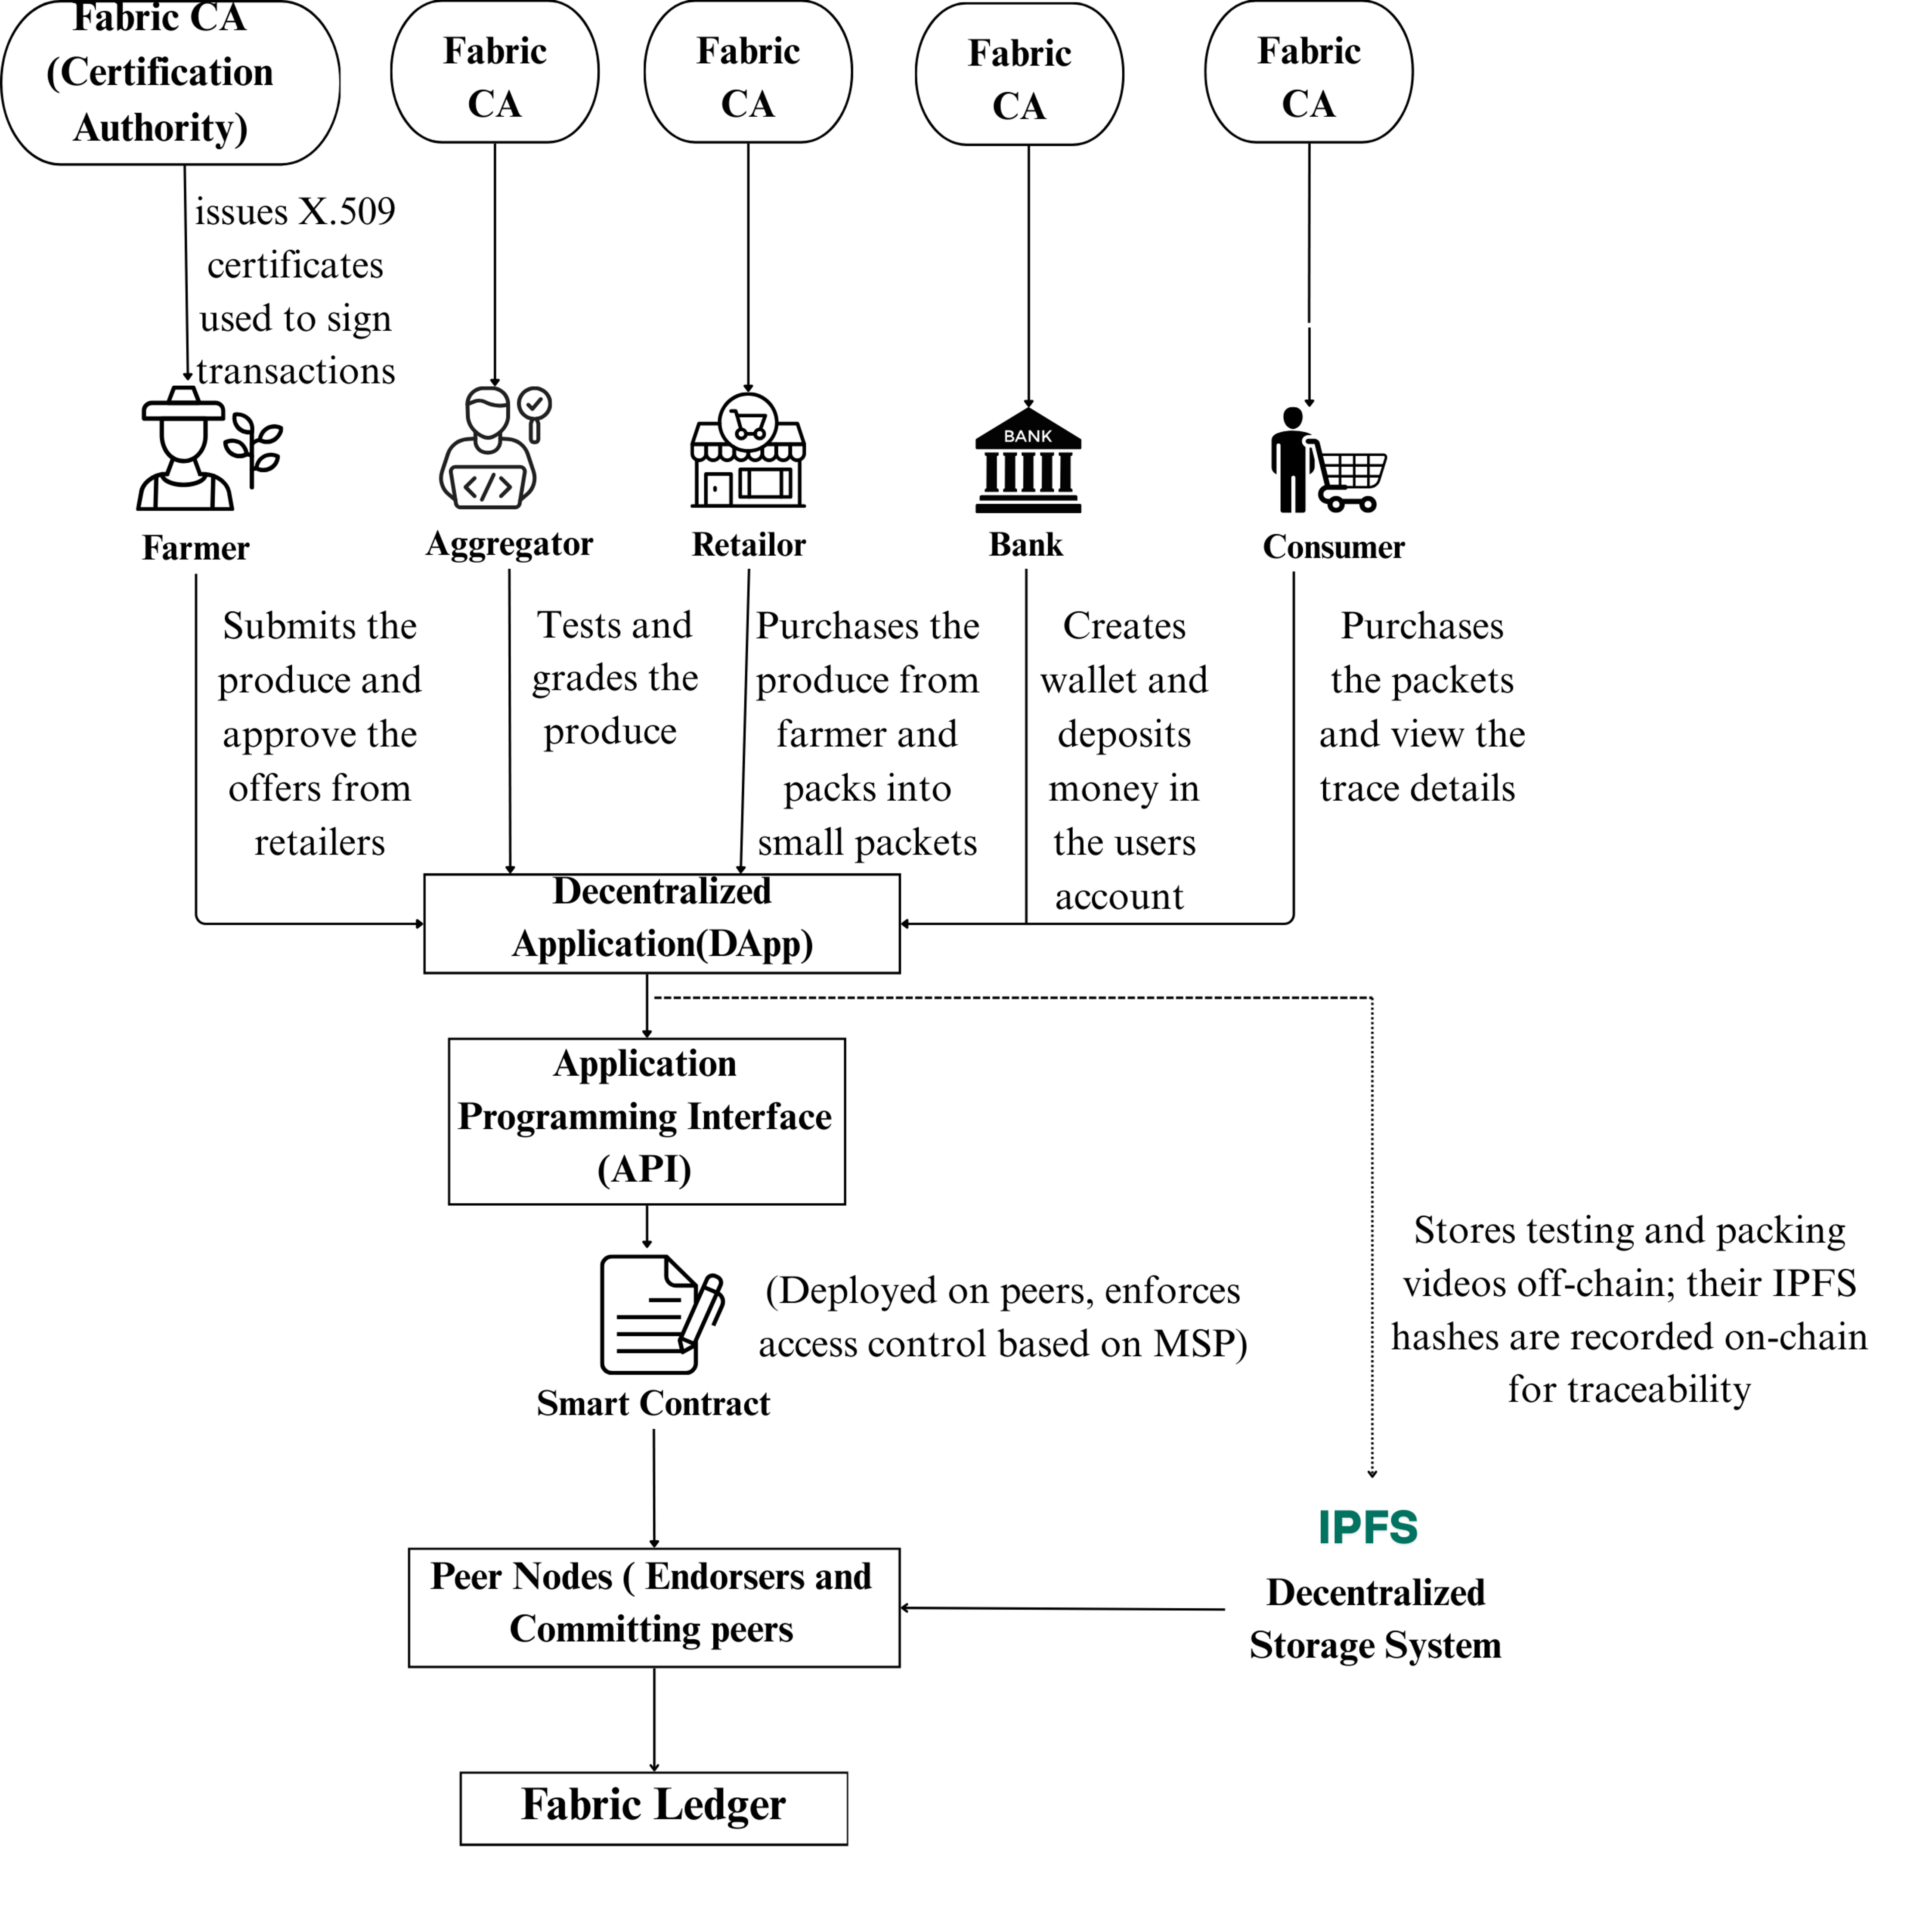
\includegraphics[width=0.9\textwidth]{Figure_1.png}
	\caption{System overview of the proposed agricultural supply chain platform}
	\label{fig:system_overview}
\end{figure}
	
	\subsection{Blockchain Network Architecture}
	
	The blockchain network was implemented using Hyperledger Fabric with five organizations: FarmersMSP, AggregatorsMSP, RetailersMSP, ConsumersMSP, and BankMSP. Each organization was configured with its own peer, MSP, and certificate authority. The organizations interact through a common channel, while CouchDB stores the world state. The network was created by extending the Fabric test network using customized Docker Compose, crypto-configuration, and channel configuration files. Raft was used as the ordering mechanism.
	
	
	\begin{figure}[htbp]
		
		\centering
		
		
\includegraphics[width=0.9\textwidth]{Figure_5.png}
		
		\caption{Network Architecture}
		
		\label{fig:network_peer}
		
	\end{figure}
	
\subsection{Smart Contract Workflow}

The business logic was implemented as JavaScript chaincode. The bank creates and funds wallets using \texttt{createAccount}. Farmers submit lots via \texttt{createLot}, and aggregators update quality status using \texttt{testCoffee}. Retailers bid via \texttt{makeOffer}, and the highest bidder executes \texttt{purchaseLot}, transferring funds automatically from their wallet to the farmer's wallet. Retailers repackage purchased lots using \texttt{createPacket}. Key features include: \texttt{createWallet()} and \texttt{depositMoney()}. Farmers submit agricultural lots using \texttt{submitProduce()}, and the testing fee is transferred to the selected aggregator. Aggregators record quality test results and grading details using \texttt{testCoffee()}. Approved lots are made available for retailer offers through \texttt{makeOffer()}, and farmers accept the highest valid offer using \texttt{acceptOffer()}. Retailers then pack accepted lots into packets using \texttt{packLotIntoPackets()}, while consumers purchase packets using \texttt{purchasePacket()} and verify provenance through lifecycle query functions. The overall sequence of stakeholder actions and smart contract functions is shown in Figure~\ref{fig:chaincode_flow}.

\begin{figure}[htbp]
	\centering
	
\includegraphics[width=\textwidth]{Figure_6.png}
	\caption{Sequence of stakeholder actions and smart contract functions in the agricultural supply chain}
	\label{fig:chaincode_flow}
\end{figure}


\subsection{MVCC Conflict Vulnerabilities}

In high-throughput environments, the unoptimized chaincode is highly susceptible to Multi-Version Concurrency Control (MVCC) conflicts. Hyperledger Fabric employs an optimistic concurrency model: transactions are executed, endorsed, and ordered before validation against the ledger state. During the validation phase, if the version of a state key read during execution does not match the current committed version on the ledger, the transaction is marked invalid (MVCC \texttt{READ\_CONFLICT}) and abruptly dropped. In this supply chain design, there are two primary architectural bottlenecks where these conflicts predominantly occur:

\begin{enumerate}
    \item \textbf{Wallet Edits (\textit{submitProduce}, \textit{acceptOffer}, \textit{purchasePacket}):} Functions that facilitate financial transactions inherently invoke a shared internal \texttt{\_transfer} method. This method reads the current wallet balances of the sender and receiver, computes the new balances, and executes a \texttt{putState} operation to overwrite them. When multiple participants interact with a single entity concurrently (e.g., 50 farmers simultaneously submitting produce to a single aggregator), all 50 transactions read the exact same initial version of the aggregator's wallet key. The first transaction to successfully commit will increment the ledger version of that wallet. Consequently, the remaining 49 transactions will fail validation, severely throttling throughput.
    
    \item \textbf{Lot Highest Offer Edits (\textit{makeOffer}):} The auction mechanism allows multiple retailers to bid on an available agricultural lot concurrently. The \texttt{makeOffer} function reads the lot's current \texttt{highestOffer} parameter, validates if the new incoming bid is strictly greater, and overwrites the lot state. If multiple retailers bid on the exact same lot within the same block generation window, only the first endorsed transaction will successfully commit the updated lot state. The subsequent bids will encounter an MVCC conflict on the lot's shared composite key, causing those transactions to fail regardless of whether their bid values were objectively higher.
\end{enumerate}

These structural vulnerabilities form the foundational basis for the machine learning predictive models developed in this study, explicitly linking function complexity and hot-key density to deterministic transaction failure rates.


\section{Methodology}

\subsection{Benchmarking Setup}



The performance of the blockchain network was rigorously evaluated using Hyperledger Caliper, the industry-standard benchmarking tool for blockchain frameworks. The primary objective was to observe the dynamic shifts in transaction throughput and failure rates in response to increasing transaction send rates, fluctuating participant density, varying chaincode function complexity, and the resulting Multi-Version Concurrency Control (MVCC) hot-key contention.

\subsubsection{Transaction Loads and Workload Functions}

To capture the full spectrum of system performance—from an idle baseline to extreme network saturation—the experiments were conducted across a sequence of fixed-rate Transaction Per Second (TPS) loads: 1, 2, 4, 8, 10, 20, 50, 100, 200, 400, and 500 TPS. The default transaction duration for each load level was maintained at 5 seconds, with specific bulk operations extended to 100 seconds to ensure steady-state measurements. The benchmarking suite tested multiple distinct chaincode functions to represent real-world supply chain workflows, including \textit{testCoffee}, \textit{makeoffer}, \textit{acceptoffer}, \textit{pack}, and \textit{submitproduce}. Each of these functions possesses a different structural complexity in terms of the number of state reads and writes required, as well as the number of participants contending for the same ledger key.

\subsubsection{Strategic Participant Matrix and Dynamic Caliper Network Generation}

To evaluate the impact of concurrent user scaling without exhaustively testing redundant participant combinations, a strategic participant matrix was designed. The number of participants for key roles (e.g., Farmers, Aggregators, Retailers) was scaled across predefined thresholds: 1, 2, 5, 10, 15, 20, and 24. 

For functions requiring interactive multi-party dependencies (such as Farmers submitting produce to Aggregators), a two-dimensional participant matrix was generated. This approach ensured comprehensive coverage of both balanced and imbalanced participant distributions while avoiding redundant reverse pairs.

Caliper workers were dynamically allocated based on the specific workload parameters. For example, in a \textit{submitproduce} workload configured with 5 farmers and 24 aggregators (\textit{submitproduce\_f5\_a24}), Caliper explicitly spawned 5 parallel worker processes acting as independent farmers. During execution, each farmer process probabilistically targeted one of the 24 available aggregators, actively stressing the shared ledger state and inducing measurable MVCC conflicts on the specific aggregator hot-keys.

To optimize the benchmarking infrastructure, 
un.js dynamically generated a workload-specific Caliper network configuration file for each experimental round. This dynamic provisioning ensured that only the required organizational identities (e.g., \textit{User1} to \textit{User24} for Farmers and Retailers) were actively instantiated and loaded into memory, thereby isolating chaincode performance metrics from artificial client-side resource starvation.

\begin{table}[ht]
\centering
\caption{Benchmark Workload Configurations and Participant Mapping}
\label{tab:workload_mapping}
\resizebox{\columnwidth}{!}{%
\begin{tabular}{|l|l|l|c|}
\hline
\textbf{Workload Function} & \textbf{Primary Role} & \textbf{Caliper Workers} & \textbf{Participant Range} \\
\hline
\textit{submitproduce} & Farmers & $X$ (number of farmers) & Farmers (1 to $X$), Aggregators (1 to $Y$) \\
\textit{testCoffee} & Aggregators & $N$ (number of aggregators) & Aggregators (1 to $N$) \\
\textit{makeoffer} & Retailers & $N$ (number of retailers) & Retailers (1 to $N$) \\
\textit{acceptoffer} & Farmers & $X$ (number of farmers) & Farmers (1 to $X$), Retailers (1 to $Y$) \\
\textit{pack} & Retailers & $N$ (number of retailers) & Retailers (1 to $N$) \\
\hline
\end{tabular}%
}
\end{table}


\subsection{Machine Learning Method and Procedure}

The empirical output logs generated by Hyperledger Caliper across all benchmarking permutations were consolidated and extracted to formulate the primary dataset for the machine learning pipeline.

\subsubsection{Static Analysis of Smart Contract Function Complexity}

To precisely quantify the computational and state-interaction overhead of the chaincode, a custom static analysis pipeline (\textit{analyzeComplexity}) was developed. This tool systematically parses the smart contract source code to extract deterministic operational metrics per function, including the total number of ledger reads (\textit{getState}), ledger writes (\textit{putState}), conditional branches, and iteration loops. Most importantly, the tool explicitly identifies the exact composite keys targeted during write operations (MVCC Write Keys). By defining these structural metrics (detailed in Table \ref{tab:function_complexity}), the machine learning model can definitively correlate transaction performance with the exact number of highly contested hot-keys updated per invocation.

\begin{table}[ht]
\centering
\caption{Static Analysis of Smart Contract Function Complexity and MVCC Hot-Keys}
\label{tab:function_complexity}
\resizebox{\columnwidth}{!}{%
\begin{tabular}{|l|c|c|c|}
\hline
\textbf{Function} & \textbf{Total Reads} & \textbf{Total Writes} & \textbf{MVCC Write Keys (Hot-Keys)} \\
\hline
\textit{submitProduce} & 3 & 3 & Wallet Balance (fromKey, toKey) \\
\textit{testCoffee} & 1 & 1 & None \\
\textit{makeOffer} & 2 & 1 & lot.highestOffer \\
\textit{acceptOffer} & 3 & 3 & Wallet Balance (fromKey, toKey) \\
\textit{packLotIntoPackets} & 1 & $1+n$ & None \\
\textit{purchasePacket} & 3 & 3 & Wallet Balance (fromKey, toKey) \\
\hline
\end{tabular}%
}
\end{table}

\vspace{0.2cm}
\noindent \small{*Note: For the empirical benchmarking simulations conducted in this study, the number of packets generated per lot ($n$) during the \textit{packLotIntoPackets} function was fixed at 55.}

 
  \subsubsection{Mechanics of MVCC Hot-Key Contention}
  In Hyperledger Fabric, Multi-Version Concurrency Control (MVCC) ensures data integrity by preventing concurrent transactions from modifying the exact same ledger state simultaneously. A ``hot-key'' bottleneck occurs when multiple active clients attempt to update the same state variable (key) at the exact same moment. If multiple transactions target the same state variable in the same block window, the first transaction successfully commits, while all subsequent concurrent transactions are instantly rejected by the validation peers with an MVCC read-write conflict, resulting in transaction failure.
  
  In the context of the proposed agri-food smart contracts, these hot-key collisions mathematically dictate the failure rate and manifest in specific algorithmic patterns:
  \begin{table}[ht]
\centering
\caption{Selected Features for Machine Learning Prediction}
\label{tab:feature_selection}
\resizebox{\columnwidth}{!}{%
\begin{tabular}{|p{0.25\linewidth}|p{0.7\linewidth}|}
\hline
\textbf{Feature} & \textbf{Description \& Rationale} \\
\hline
\textbf{Transaction Send Rate (Load)} & The targeted number of transactions submitted per second. \\
\hline
\textbf{Number of Caliper Workers} & The number of parallel client workers actively submitting transactions simultaneously, directly dictating concurrent thread pressure. \\
\hline
\textbf{Participant Density} & The explicit count of active Farmers, Aggregators, Retailers, Consumers, and Bank Users interacting with the smart contract. \\
\hline
\textbf{Number of Ledger Writes} & Extracted via static analysis, representing baseline structural complexity. Allows mathematical correlation of algorithmic topology to failure vulnerabilities rather than relying on categorical function names. \\
\hline
\textbf{Hot-Key Participant Count} & A derived metric quantifying severity of concurrent operations on shared state keys (e.g., competing retailers bidding on a single lot, or simultaneous wallet balance edits during settlements). The total count of participants interacting with these precise hot-keys directly mathematically dictates the probability of an MVCC read-write conflict and transaction failure. \\
\hline
\end{tabular}%
}
\end{table}

To provide a comprehensive dataset for the machine learning model, the benchmarking framework generated permutations across these features using the parameter ranges defined in Table \ref{tab:experimental_ranges}.

\begin{table}[ht]
\centering
\caption{Experimental Benchmarking Parameter Ranges}
\label{tab:experimental_ranges}
\resizebox{\columnwidth}{!}{%
\begin{tabular}{|l|l|}
\hline
\textbf{Experimental Parameter} & \textbf{Evaluated Range / Values} \\
\hline
Transaction Send Rate (TPS) & 1, 2, 4, 8, 10, 20, 50, 100, 200, 400, 500 \\
Number of Caliper Workers & 1, 2, 5, 10, 15, 20, 24 \\
Participant Density Matrix & (1,1), (1,2), (1,5), (2,2), (2,5), (5,5) ... up to (24,24) \\
Transactions per Round & 500 fixed transactions per permutation \\
Workload Duration & Dynamic based on TPS, with specific caps (e.g., 100s) \\

\hline
\end{tabular}%
}
\end{table}


\begin{table}[ht]
\centering
\caption{Concurrent Hot-Key Contention Scaling Matrix across Participant Densities}
\label{tab:hotkey_scaling}
\resizebox{\columnwidth}{!}{%
\begin{tabular}{|c|c|c|c|}
\hline
\textbf{\textit{submitProduce} Hot-Keys} & \textbf{\textit{makeOffer} Hot-Keys} & \textbf{\textit{acceptOffer} Hot-Keys} & \textbf{\textit{purchasePacket} Hot-Keys} \\
\hline
2 (1 Farmer, 1 Aggregator) & 1 Lot (1 Retailer competing) & 2 (1 Farmer, 1 Retailer) & 2 (1 Consumer, 1 Retailer) \\
8 (4 Farmers, 4 Aggregators) & 1 Lot (4 Retailers competing) & 8 (4 Farmers, 4 Retailers) & 8 (4 Consumers, 4 Retailers) \\
20 (10 Farmers, 10 Aggregators) & 1 Lot (10 Retailers competing) & 20 (10 Farmers, 10 Retailers) & 20 (10 Consumers, 10 Retailers) \\
30 (15 Farmers, 15 Aggregators) & 1 Lot (15 Retailers competing) & 30 (15 Farmers, 15 Retailers) & 30 (15 Consumers, 15 Retailers) \\
40 (20 Farmers, 20 Aggregators) & 1 Lot (20 Retailers competing) & 40 (20 Farmers, 20 Retailers) & 40 (20 Consumers, 20 Retailers) \\
48 (24 Farmers, 24 Aggregators)& 1 Lot (24 Retailers competing) & 48 (24 Farmers, 24 Retailers) & 48 (24 Consumers, 24 Retailers) \\
\hline
\end{tabular}%
}
\end{table}
\subsubsection{Predictive Modeling and Baseline Comparison}

To map the relationship between these system variables and the observed chaincode behavior, five distinct machine learning regression architectures were evaluated:
\begin{table}[ht]
\centering
\caption{Evaluated Machine Learning Regression Architectures}
\label{tab:ml_models}
\resizebox{\columnwidth}{!}{%
\begin{tabular}{|p{0.3\linewidth}|p{0.2\linewidth}|p{0.5\linewidth}|}
\hline
\textbf{Predictive Model} & \textbf{Architecture Class} & \textbf{Description \& Rationale} \\
\hline
\textbf{Linear Regression} & Baseline & Linear baseline; tested to prove incapability of modeling discrete, non-linear MVCC state ceilings. \\
\hline
\textbf{Support Vector Regressor (SVR)} & Distance-based & Evaluates structural mapping of continuous variables in high-dimensional space. \\
\hline
\textbf{Multi-Layer Perceptron (MLP)} & Neural Network & Capable of mapping non-linear boundaries but inherently blurs discrete integer thresholds and lacks feature interpretability. \\
\hline
\textbf{Random Forest Regressor} & Tree Ensemble & Aggregates multiple independent decision trees to reduce prediction variance. \\
\hline
\textbf{a Random Forest ensemble} & Boosting Ensemble & Sequentially builds trees to explicitly correct residual errors; natively provides transparent feature importance extraction. \\
\hline
\end{tabular}%
}
\end{table}

The selection of a Random Forest ensemble as the primary predictive architecture was driven by the unique failure mechanics of Hyperledger Fabric. Blockchain performance degradation---specifically MVCC read-write conflicts and throughput saturation---does not scale linearly. A network remains perfectly stable until a specific structural limit is hit (e.g., a critical mass of concurrent hot-key collisions or resource exhaustion), at which point performance drops off a severe "cliff" (jumping abruptly from 0\% to high failure rates). Linear mapping models like Linear Regression and Support Vector Regression (SVR) are fundamentally incapable of modeling these strict, sudden thresholds. While Neural Networks (MLPs) can model non-linear boundaries, they inherently blur discrete integer transitions and lack interpretability. Conversely, tree-based ensemble methods like Random Forest create distinct conditional splits (e.g., IF Hot-Keys > 2 AND Load > 300 $\rightarrow$ Failure = 85\%), perfectly mimicking the conditional transaction validation logic of blockchain state machines. Furthermore, Random Forest natively calculates feature importance through independent bagging (Feature Importance), allowing for the extraction of mathematical proof regarding which structural parameters act as the primary bottlenecks, making it the optimal and most interpretable choice for this study.

Crucially, rather than predicting the absolute number of failed transactions (which is artificially biased by the total number of transactions sent), the models were trained to predict the precise \textit{Failure Rate} (the percentage of failed transactions over the total submitted), alongside the successfully achieved system \textit{Throughput}.

\subsection{Data Collection and Feature Selection}
The dataset's features were carefully selected to capture the nonlinear interactions inherent in blockchain architecture that directly trigger transaction failures. Because MVCC failures in Hyperledger Fabric are predominantly caused by concurrent read/write operations on identical state keys, the selected independent variables explicitly quantified both the computational load and the specific state-write dependencies. The primary features included:

\begin{table}[ht]
\centering
\caption{Selected Features for Machine Learning Prediction}
\label{tab:feature_selection}
\resizebox{\columnwidth}{!}{%
\begin{tabular}{|p{0.25\linewidth}|p{0.7\linewidth}|}
\hline
\textbf{Feature} & \textbf{Description \& Rationale} \\
\hline
\textbf{Transaction Send Rate (Load)} & The targeted number of transactions submitted per second. \\
\hline
\textbf{Number of Caliper Workers} & The number of parallel client workers actively submitting transactions simultaneously, directly dictating concurrent thread pressure. \\
\hline
\textbf{Participant Density} & The explicit count of active Farmers, Aggregators, Retailers, Consumers, and Bank Users interacting with the smart contract. \\
\hline
\textbf{Number of Ledger Writes} & Extracted via static analysis, representing baseline structural complexity. Allows mathematical correlation of algorithmic topology to failure vulnerabilities rather than relying on categorical function names. \\
\hline
\textbf{Hot-Key Participant Count} & A derived metric quantifying severity of concurrent operations on shared state keys (e.g., competing retailers bidding on a single lot, or simultaneous wallet balance edits during settlements). The total count of participants interacting with these precise hot-keys directly mathematically dictates the probability of an MVCC read-write conflict and transaction failure. \\
\hline
\end{tabular}%
}
\end{table}

To provide a comprehensive dataset for the machine learning model, the benchmarking framework generated permutations across these features using the parameter ranges defined in Table \ref{tab:experimental_ranges}.

\section{Results and Discussion}
\subsection{Empirical Network Performance Analysis}
Each core function was evaluated independently under varying send rates using Hyperledger Caliper. The tested functions included \textit{submitProduce()}, \textit{testCoffee()}, \textit{makeOffer()}, \textit{acceptOffer()}, \textit{packLotIntoPackets()}, and \textit{purchasePacket()}. The objective was to empirically quantify the architectural limits of the smart contracts prior to applying predictive machine learning.

\subsubsection{Throughput and Latency Scalability}
As visualized in Figure \ref{fig:throughput-plot} and Figure \ref{fig:latency-plot}, the network's throughput scaling is directly dictated by the algorithmic complexity of the invoked function. Under low concurrent loads (50-100 TPS), all functions scale near-linearly. However, as the transaction send rate accelerates toward 500 TPS, severe performance divergence occurs. Lightweight functions requiring minimal state modifications, such as \textit{makeOffer()} and \textit{testCoffee()}, demonstrate exceptional resilience. At 500 TPS, \textit{makeOffer()} achieved the best scalability among the tested write functions, maintaining very low average latency and reaching a maximum throughput of over 400 TPS. This result reflects its highly optimized design, requiring only a single ledger write to update the lot's highest offer parameter.

\begin{figure}[ht]
    \centering
    \begin{minipage}[b]{0.48\textwidth}
        \centering
        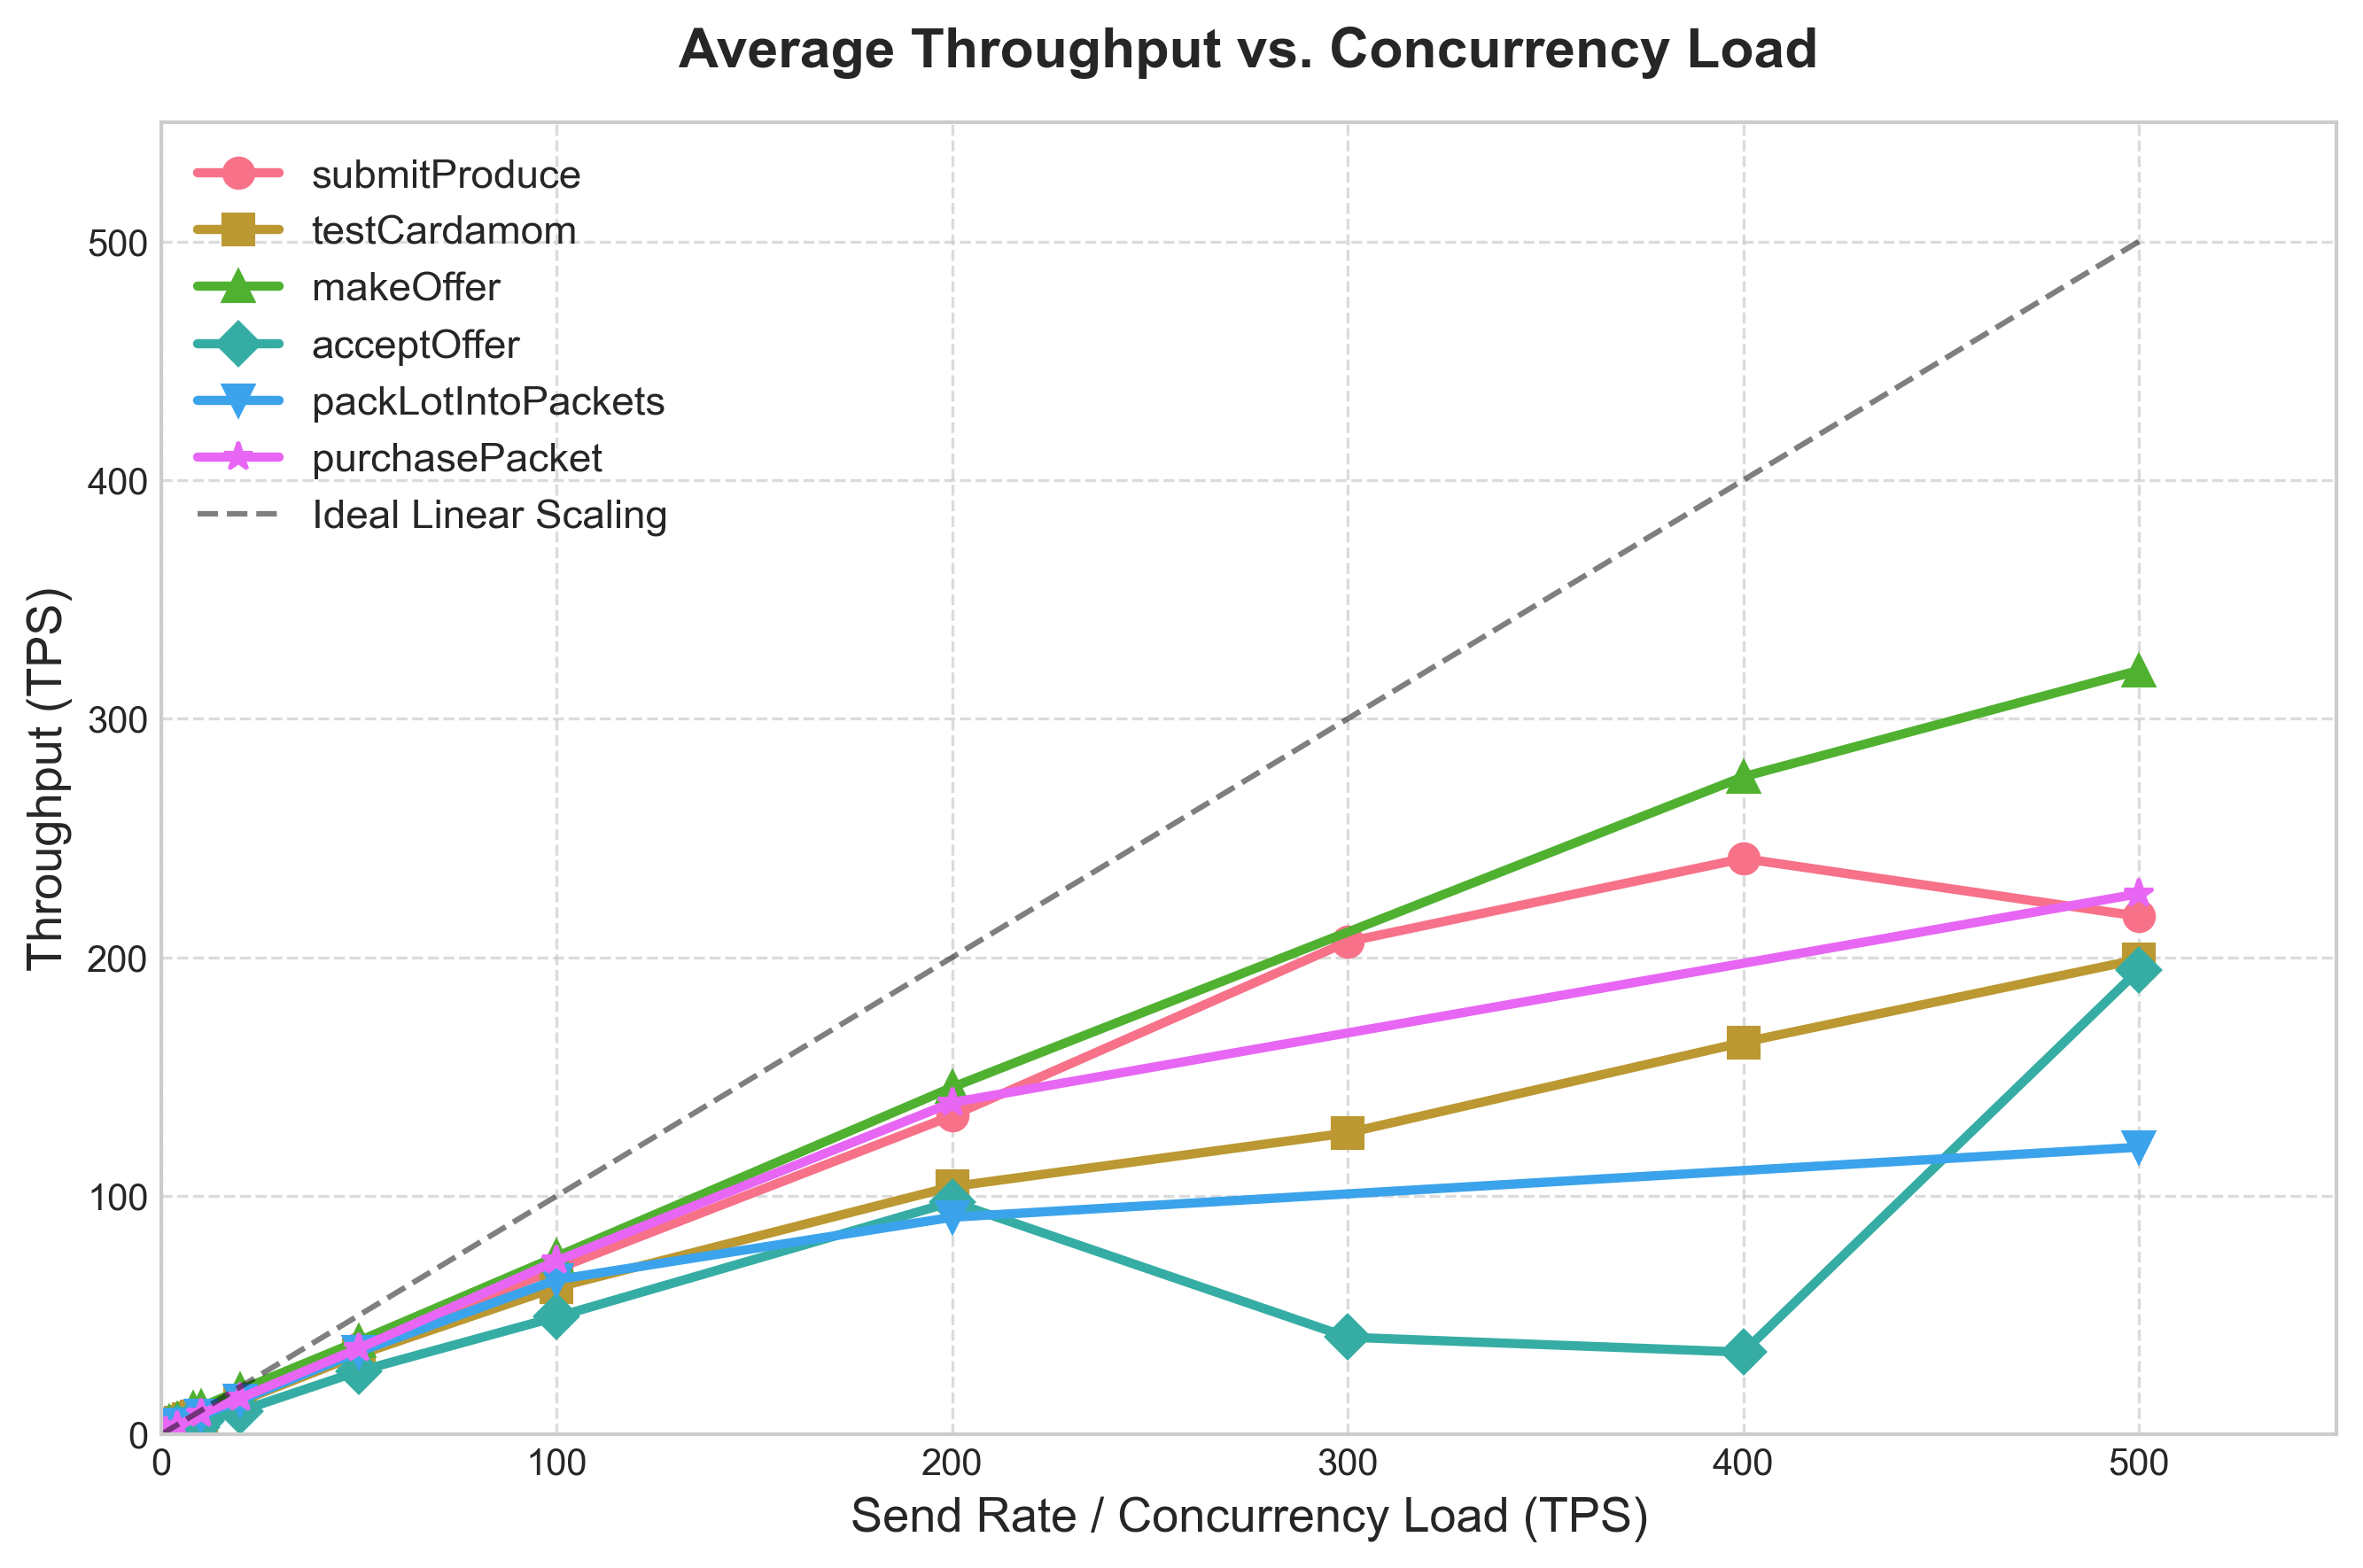
\includegraphics[width=\textwidth]{throughput_plot.png}
        \caption{Average Throughput across varying transaction loads.}
        \label{fig:throughput-plot}
    \end{minipage}
    \hfill
    \begin{minipage}[b]{0.48\textwidth}
        \centering
        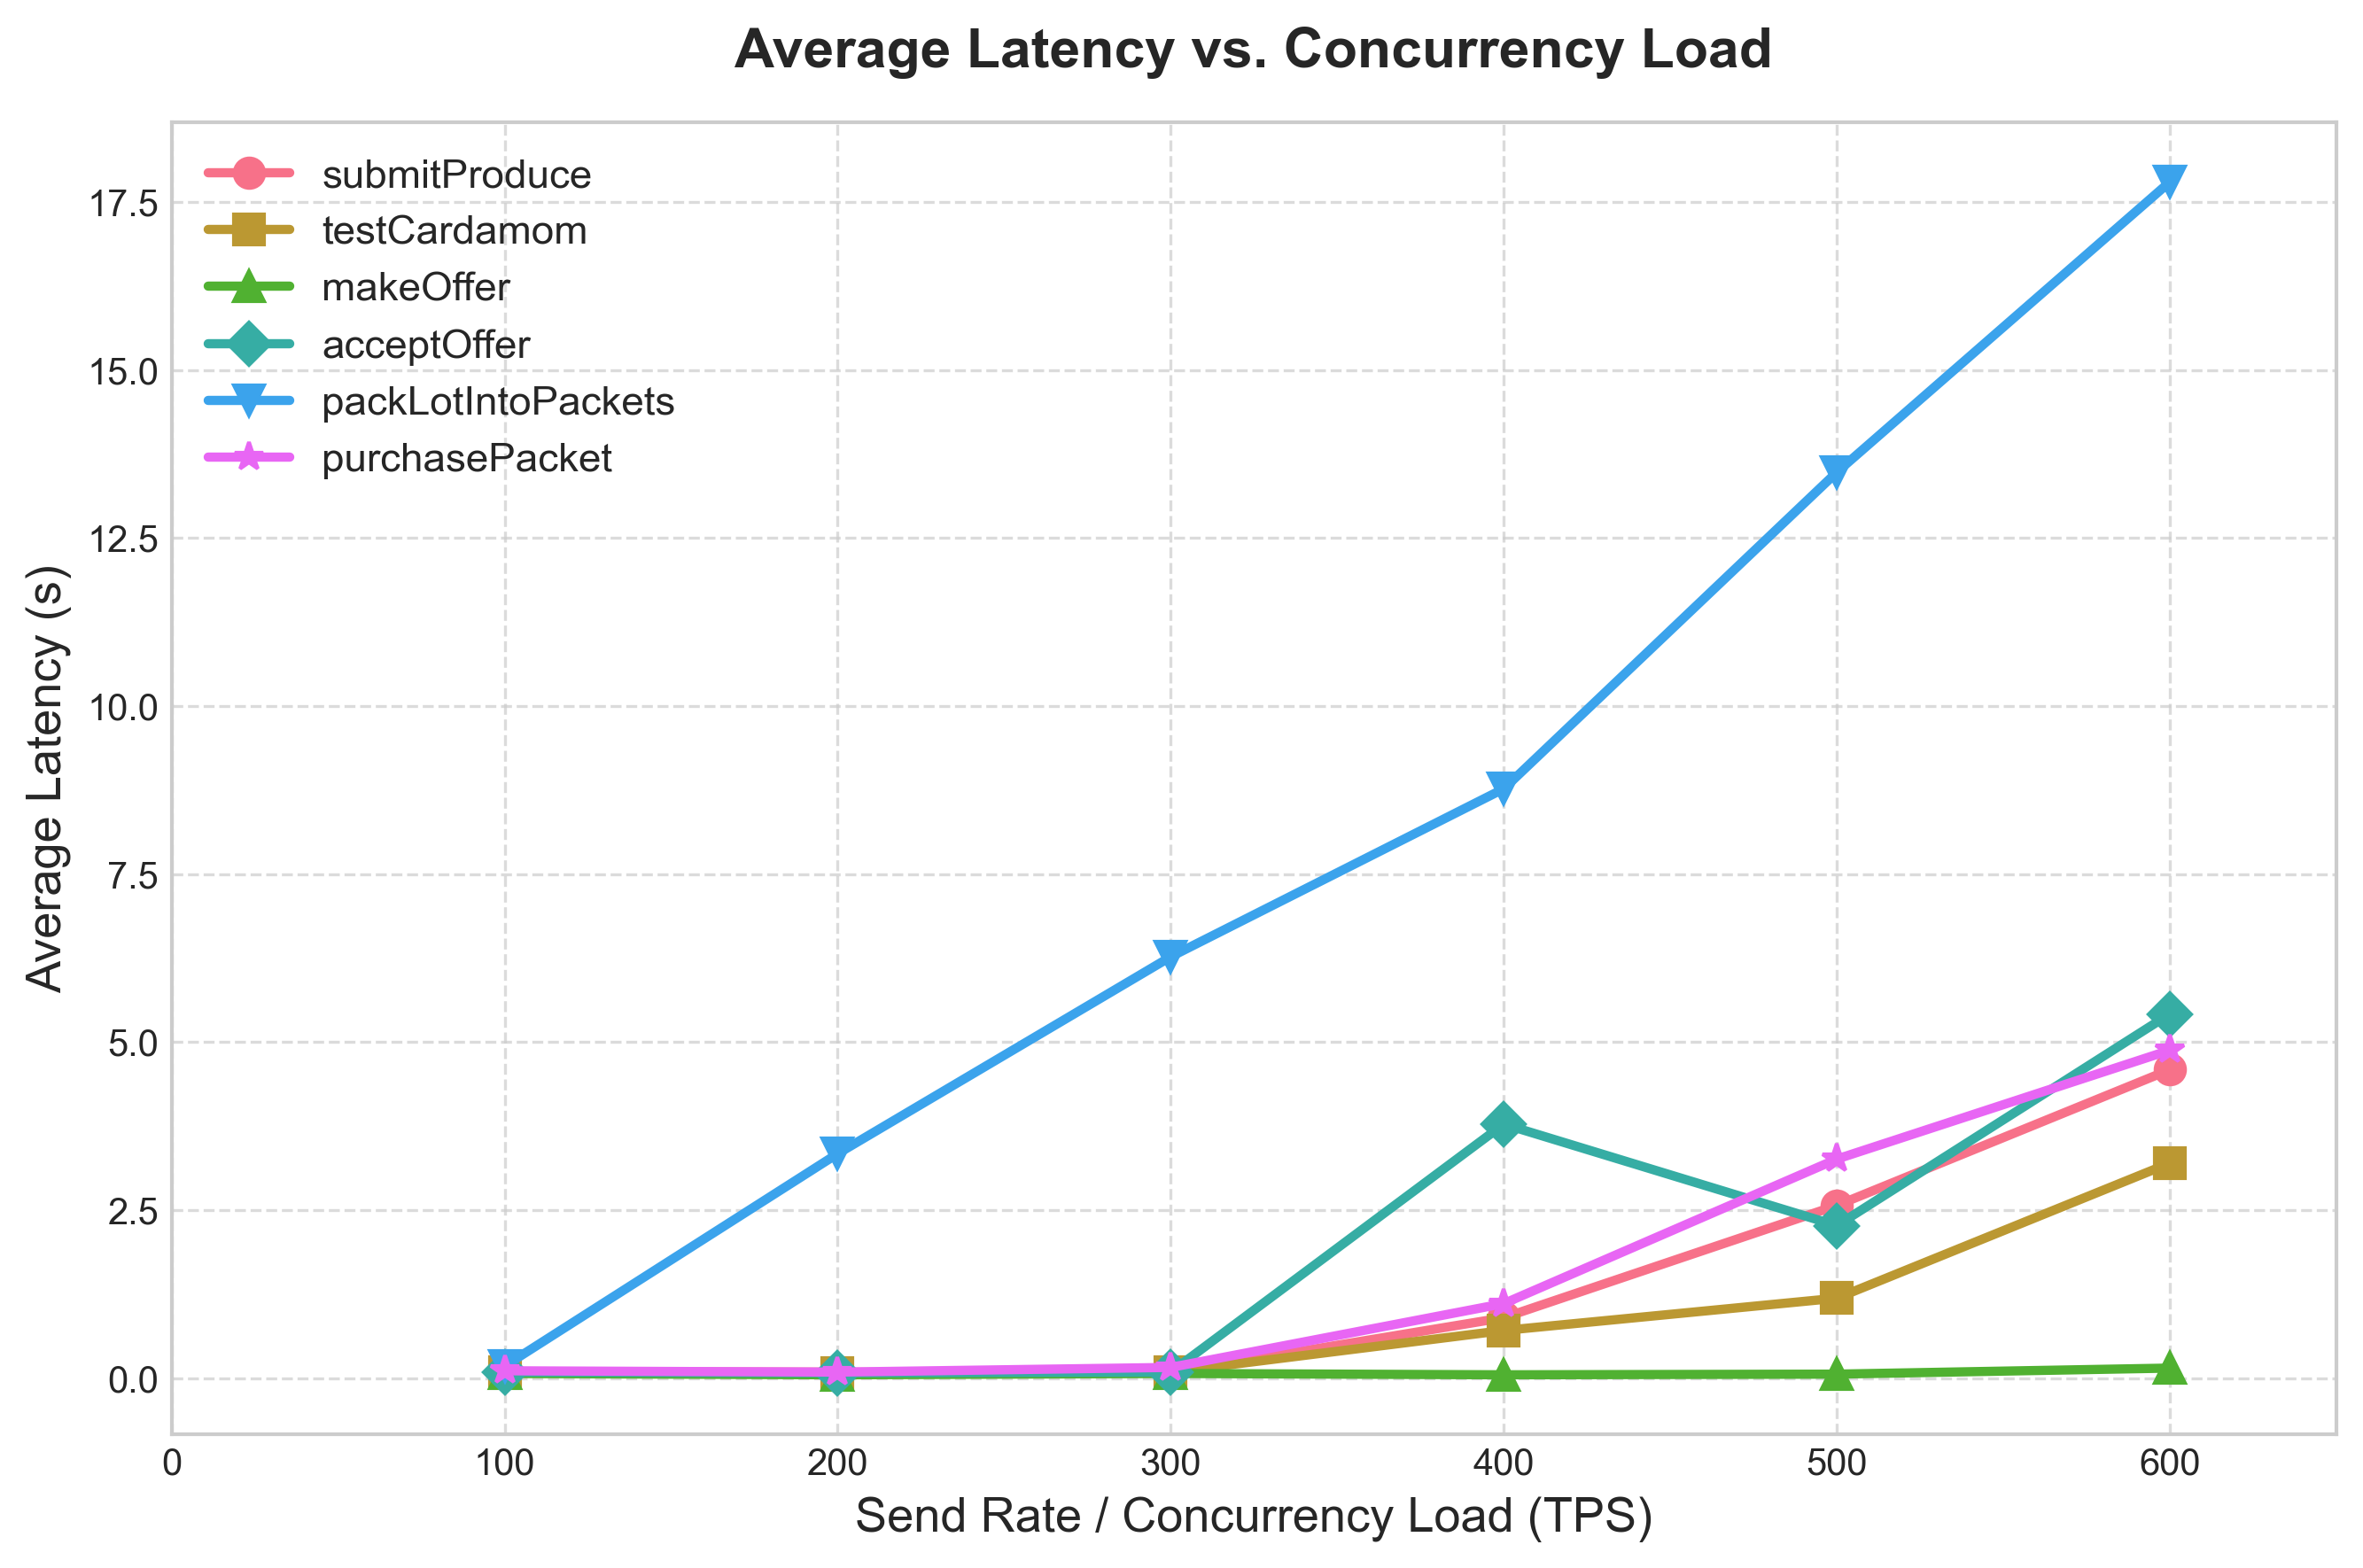
\includegraphics[width=\textwidth]{latency_plot.png}
        \caption{Average Latency across varying transaction loads.}
        \label{fig:latency-plot}
    \end{minipage}
\end{figure}

\subsubsection{Impact of Ledger Write Complexity}
Conversely, functions with heavier structural payloads exhibited aggressive performance ceilings. As demonstrated in Figure \ref{fig:throughput-writes} and Figure \ref{fig:latency-writes}, there is a strict inverse correlation between Ledger Write Complexity and sustained throughput at peak loads. The \textit{packLotIntoPackets()} function---which executes an intensive $1+n$ sequential ledger writes to generate individual produce packets---hit a hard throughput ceiling of approximately 140 TPS. The sheer volume of key-value writes per transaction overwhelmed the Fabric endorsement and commit phases, causing average latency to spike exponentially compared to the simpler functions.

\begin{figure}[ht]
    \centering
    \begin{minipage}[b]{0.48\textwidth}
        \centering
        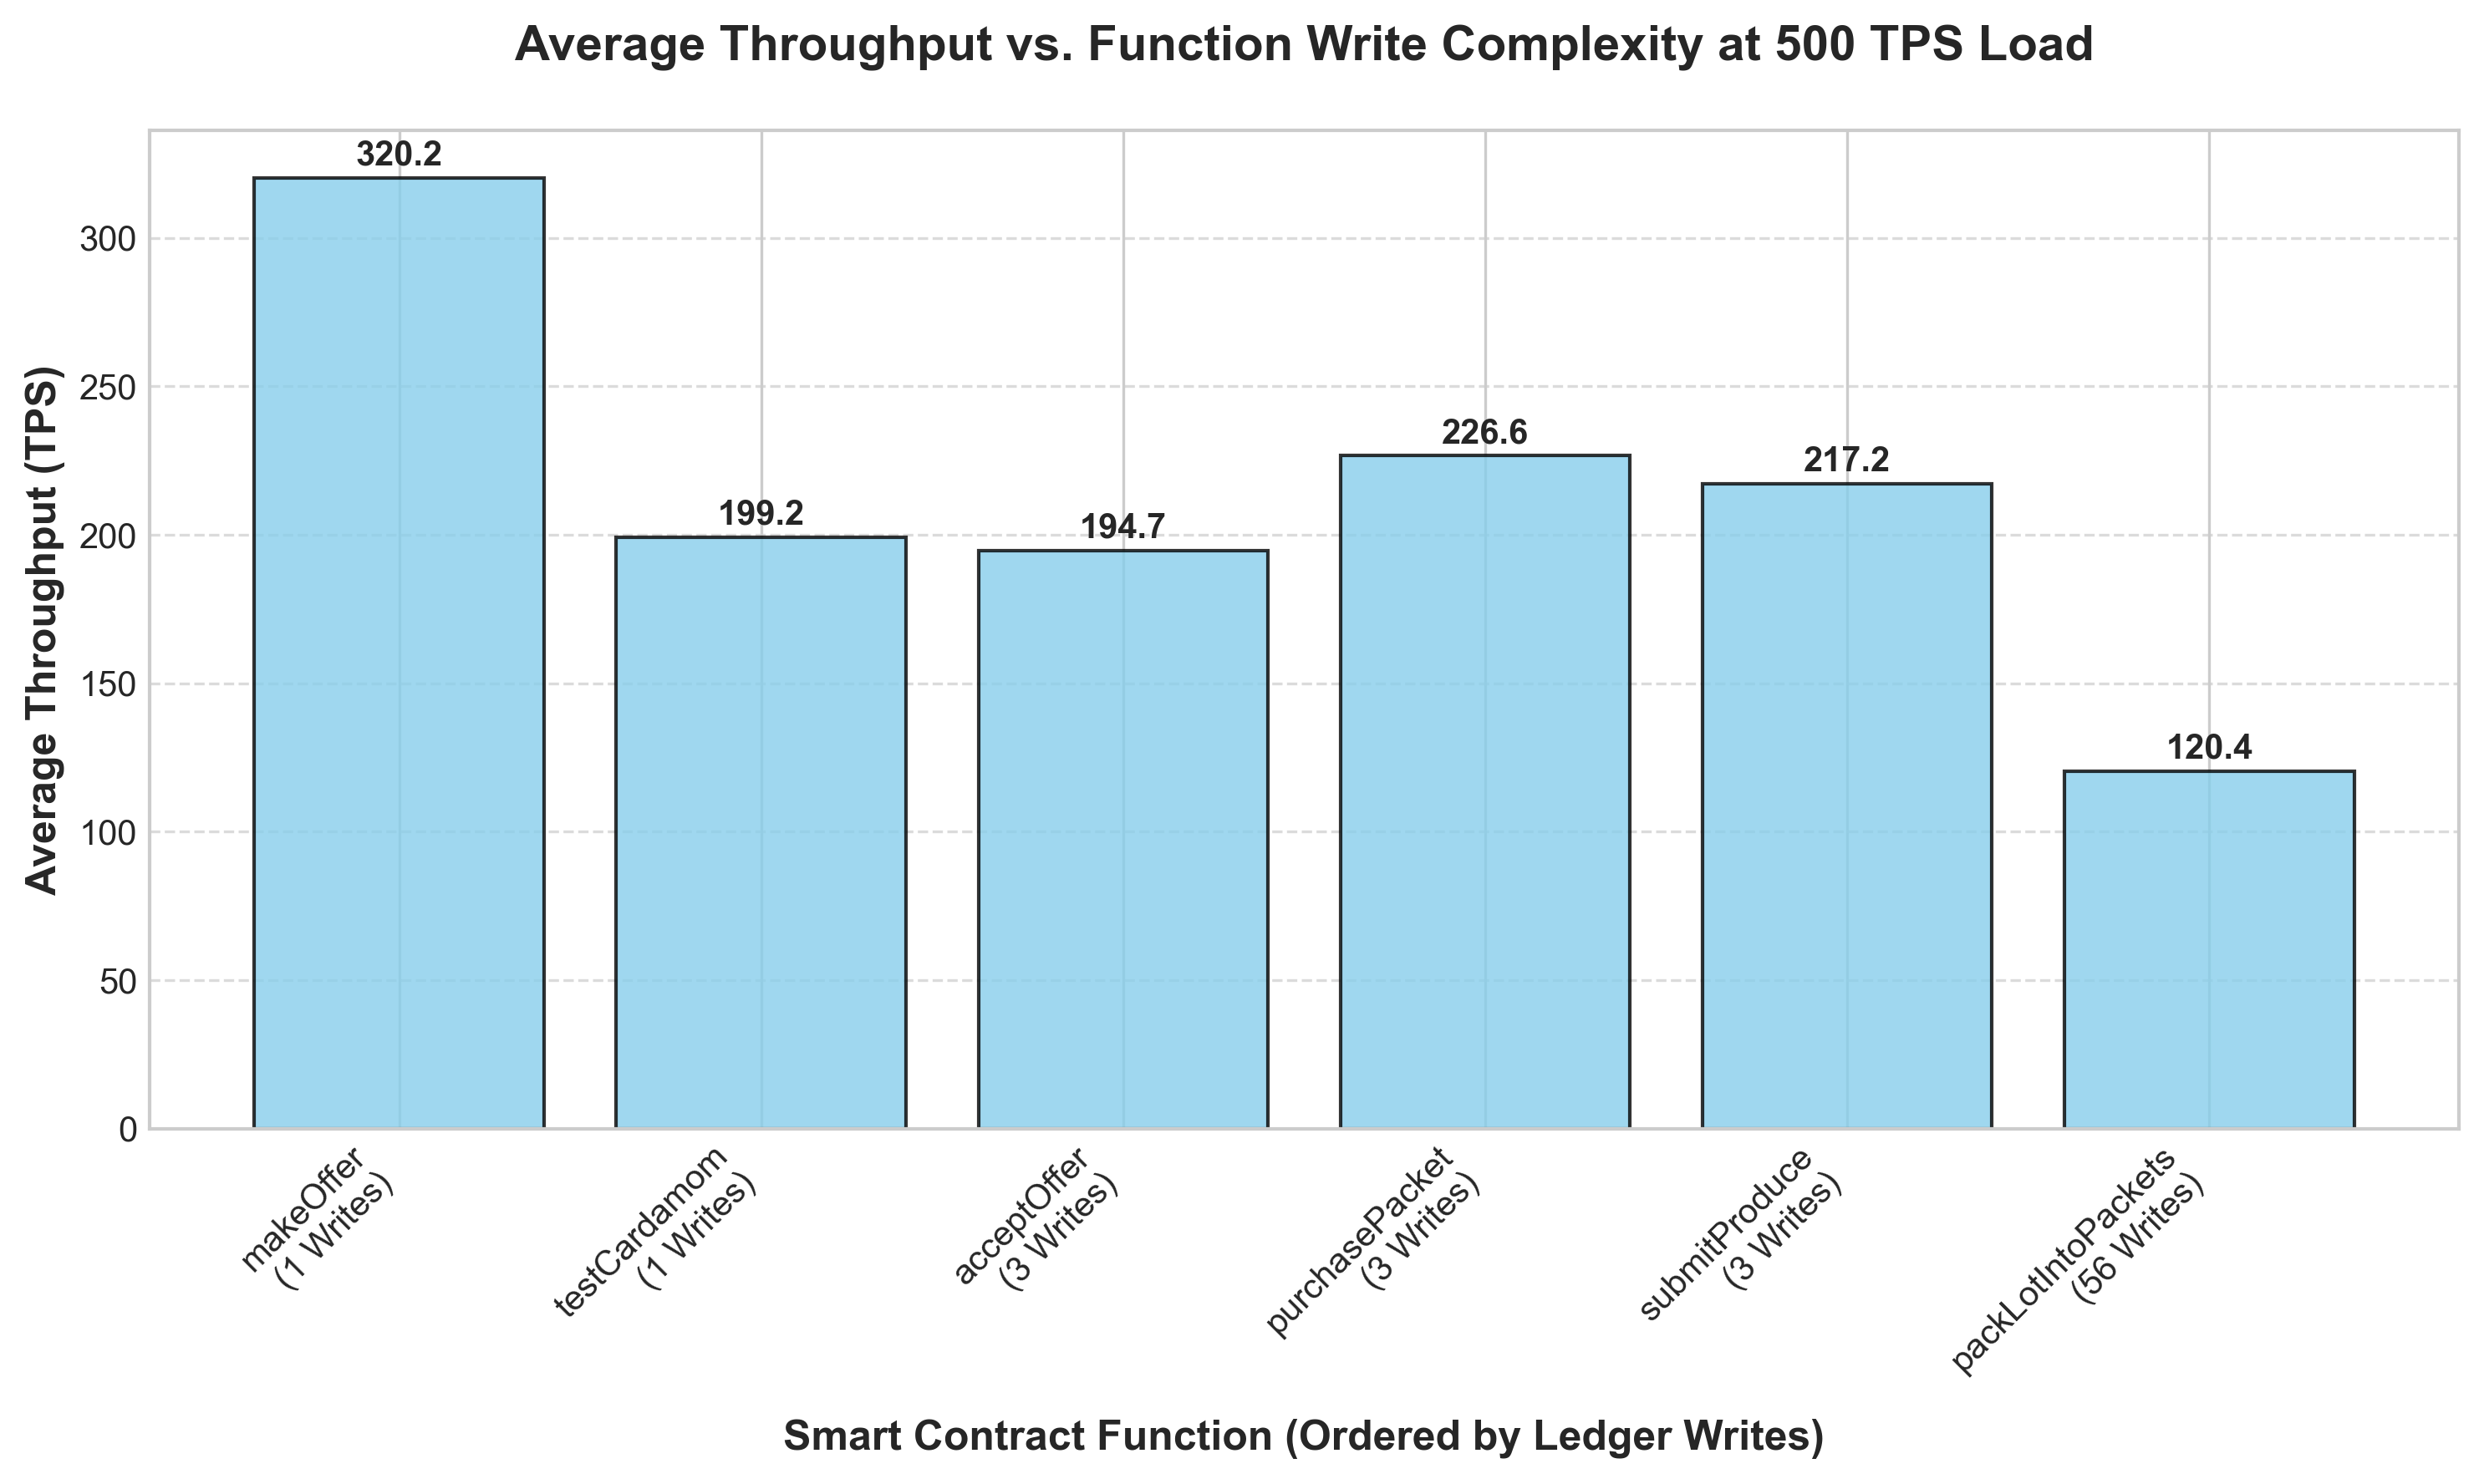
\includegraphics[width=\textwidth]{throughput_writes_500.png}
        \caption{Average Throughput vs. Write Complexity at 500 TPS.}
        \label{fig:throughput-writes}
    \end{minipage}
    \hfill
    \begin{minipage}[b]{0.48\textwidth}
        \centering
        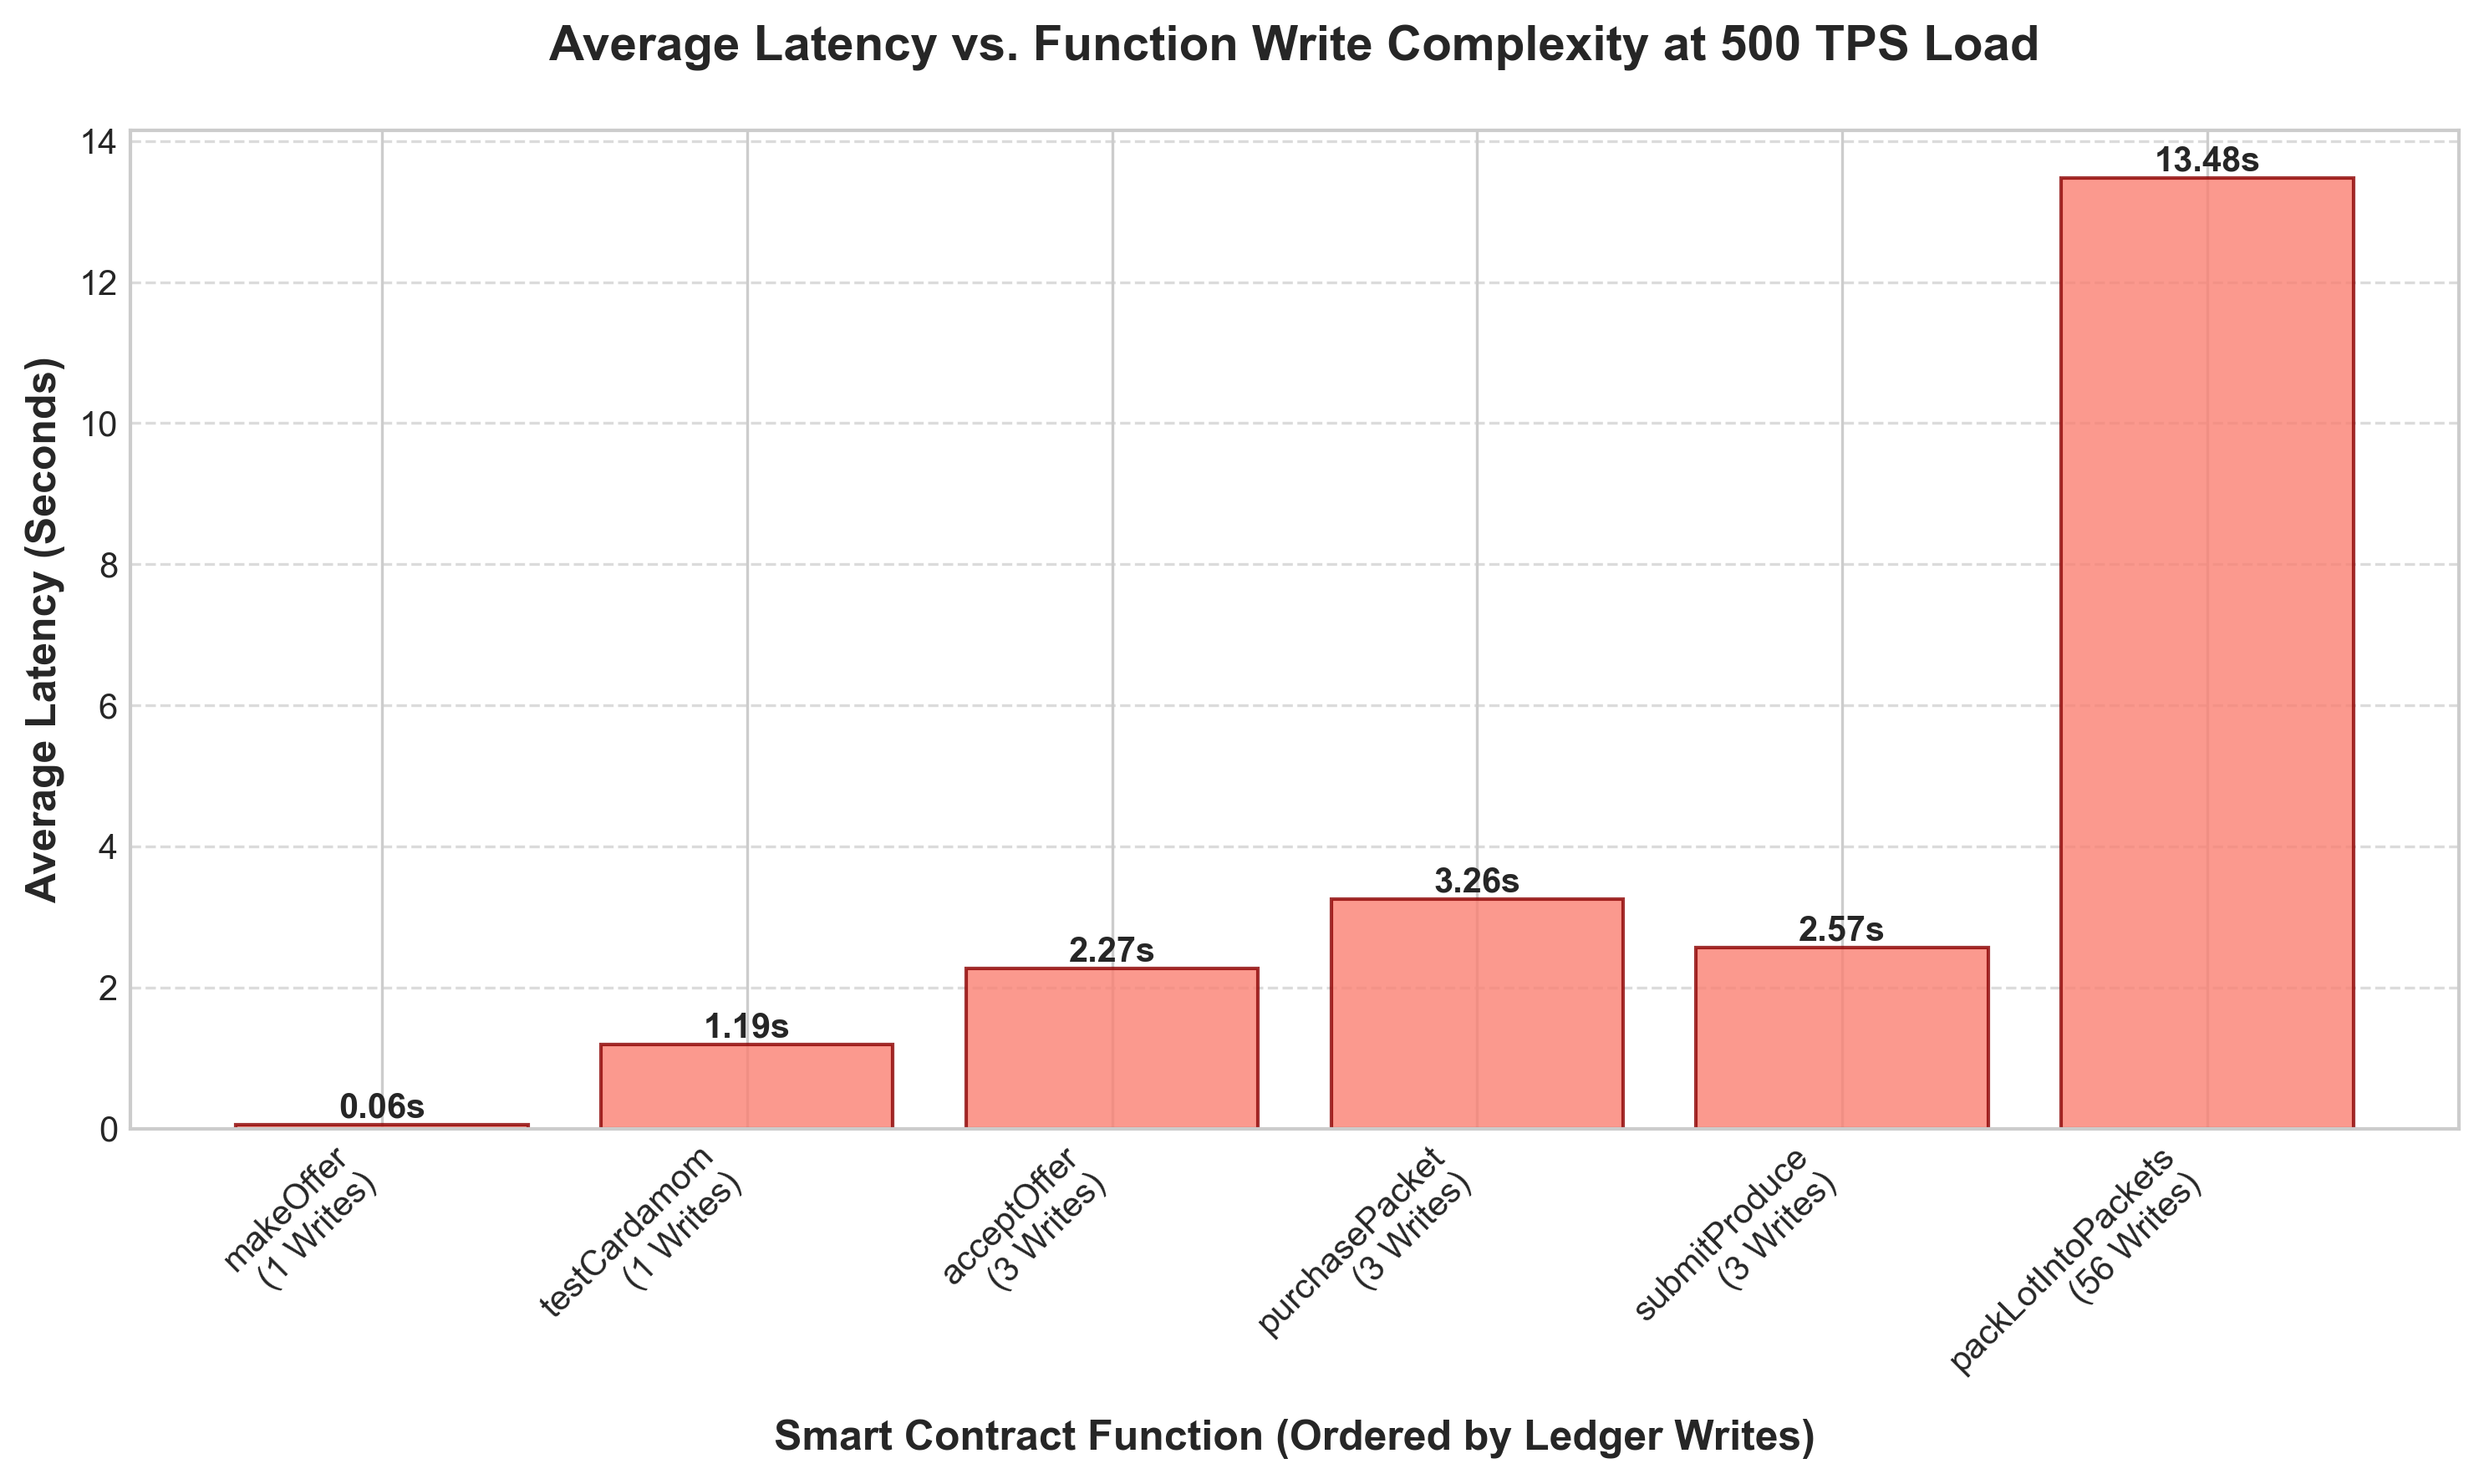
\includegraphics[width=\textwidth]{latency_writes_500.png}
        \caption{Average Latency vs. Write Complexity at 500 TPS.}
        \label{fig:latency-writes}
    \end{minipage}
\end{figure}

\subsubsection{MVCC State Contention Limits}
Finally, intermediate functions requiring complex financial settlements between two distinct participants (\textit{submitProduce()}, \textit{acceptOffer()}, and \textit{purchasePacket()}) sat firmly in the middle of the performance spectrum. These functions generally capped between 200 and 250 TPS. While they required fewer raw ledger writes than the packing function, their reliance on overlapping participant wallet updates caused severe Multi-Version Concurrency Control (MVCC) read-write conflicts on shared assets, forcing the validation peers to reject massive numbers of concurrent transactions.

To empirically validate the structural bottlenecks defined in Table \ref{tab:hotkey_scaling}, Figure \ref{fig:hotkey_failures} presents the recorded transaction failure rates plotted directly against the number of concurrent hot-key participants for four highly contended functions. As demonstrated, while higher overall transaction loads (TPS) elevate the baseline failure floor, the steepness of the failure curve is overwhelmingly driven by the specific number of participants simultaneously attempting to update a shared ledger state.

\begin{figure}[ht]
    \centering
    \begin{minipage}[b]{0.48\textwidth}
        \centering
        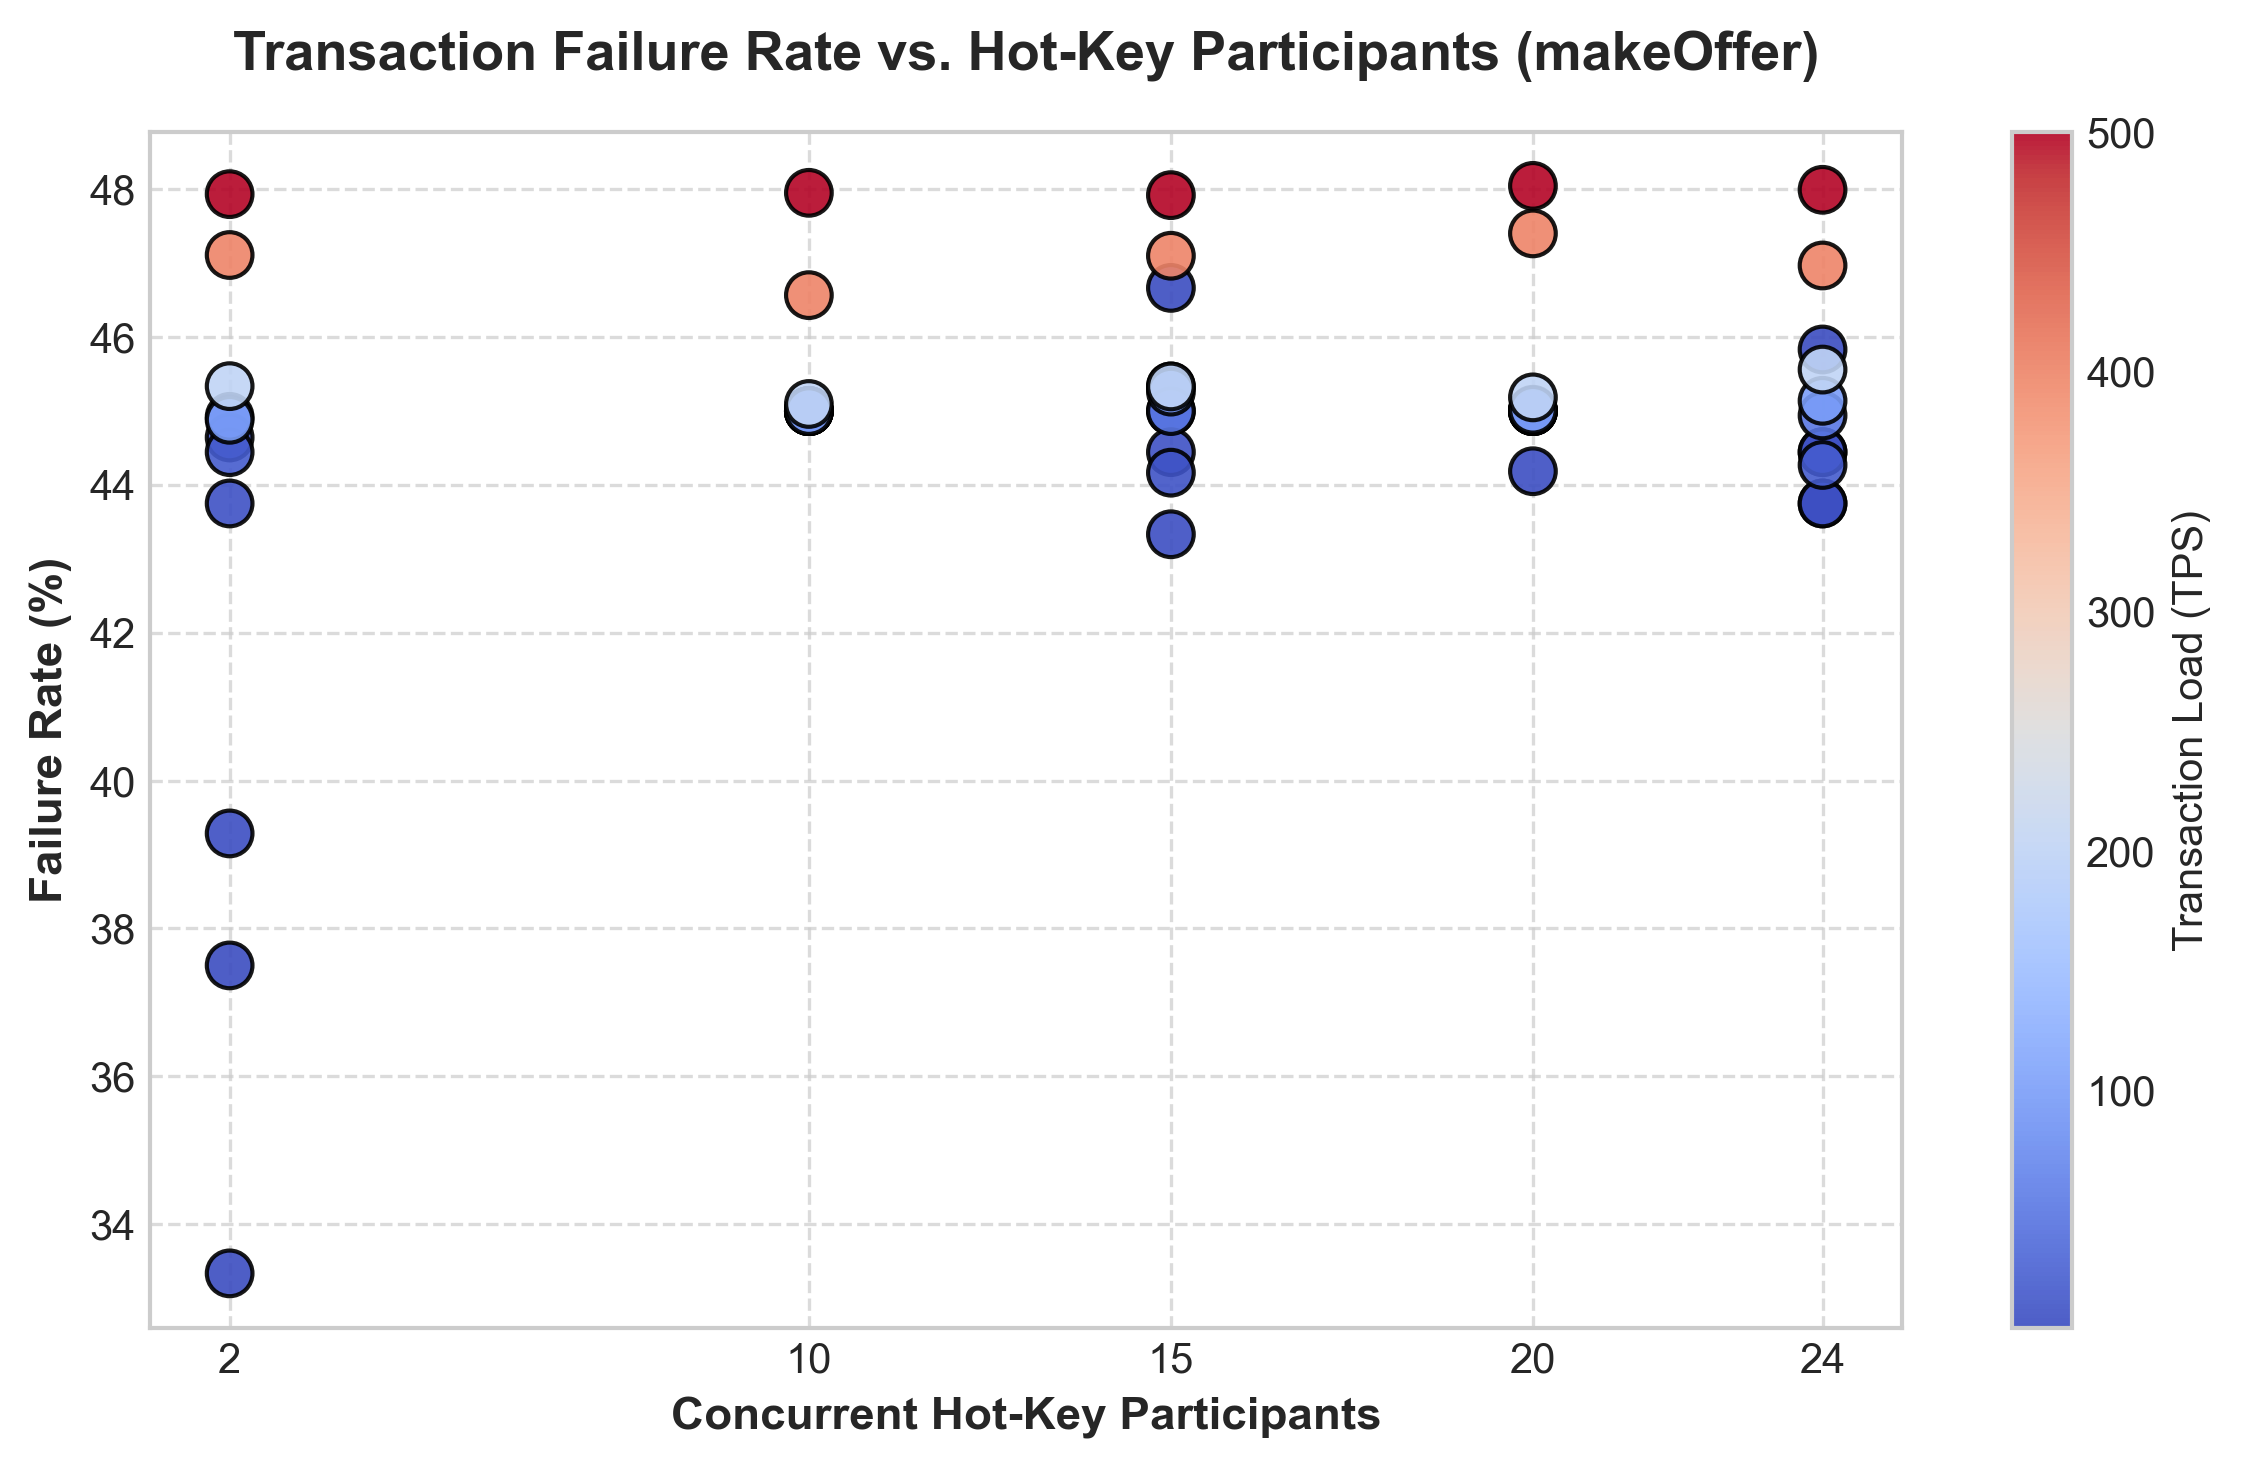
\includegraphics[width=\textwidth]{failures_vs_hotkeys_makeoffer.png}
        \caption{makeOffer}
    \end{minipage}
    \hfill
    \begin{minipage}[b]{0.48\textwidth}
        \centering
        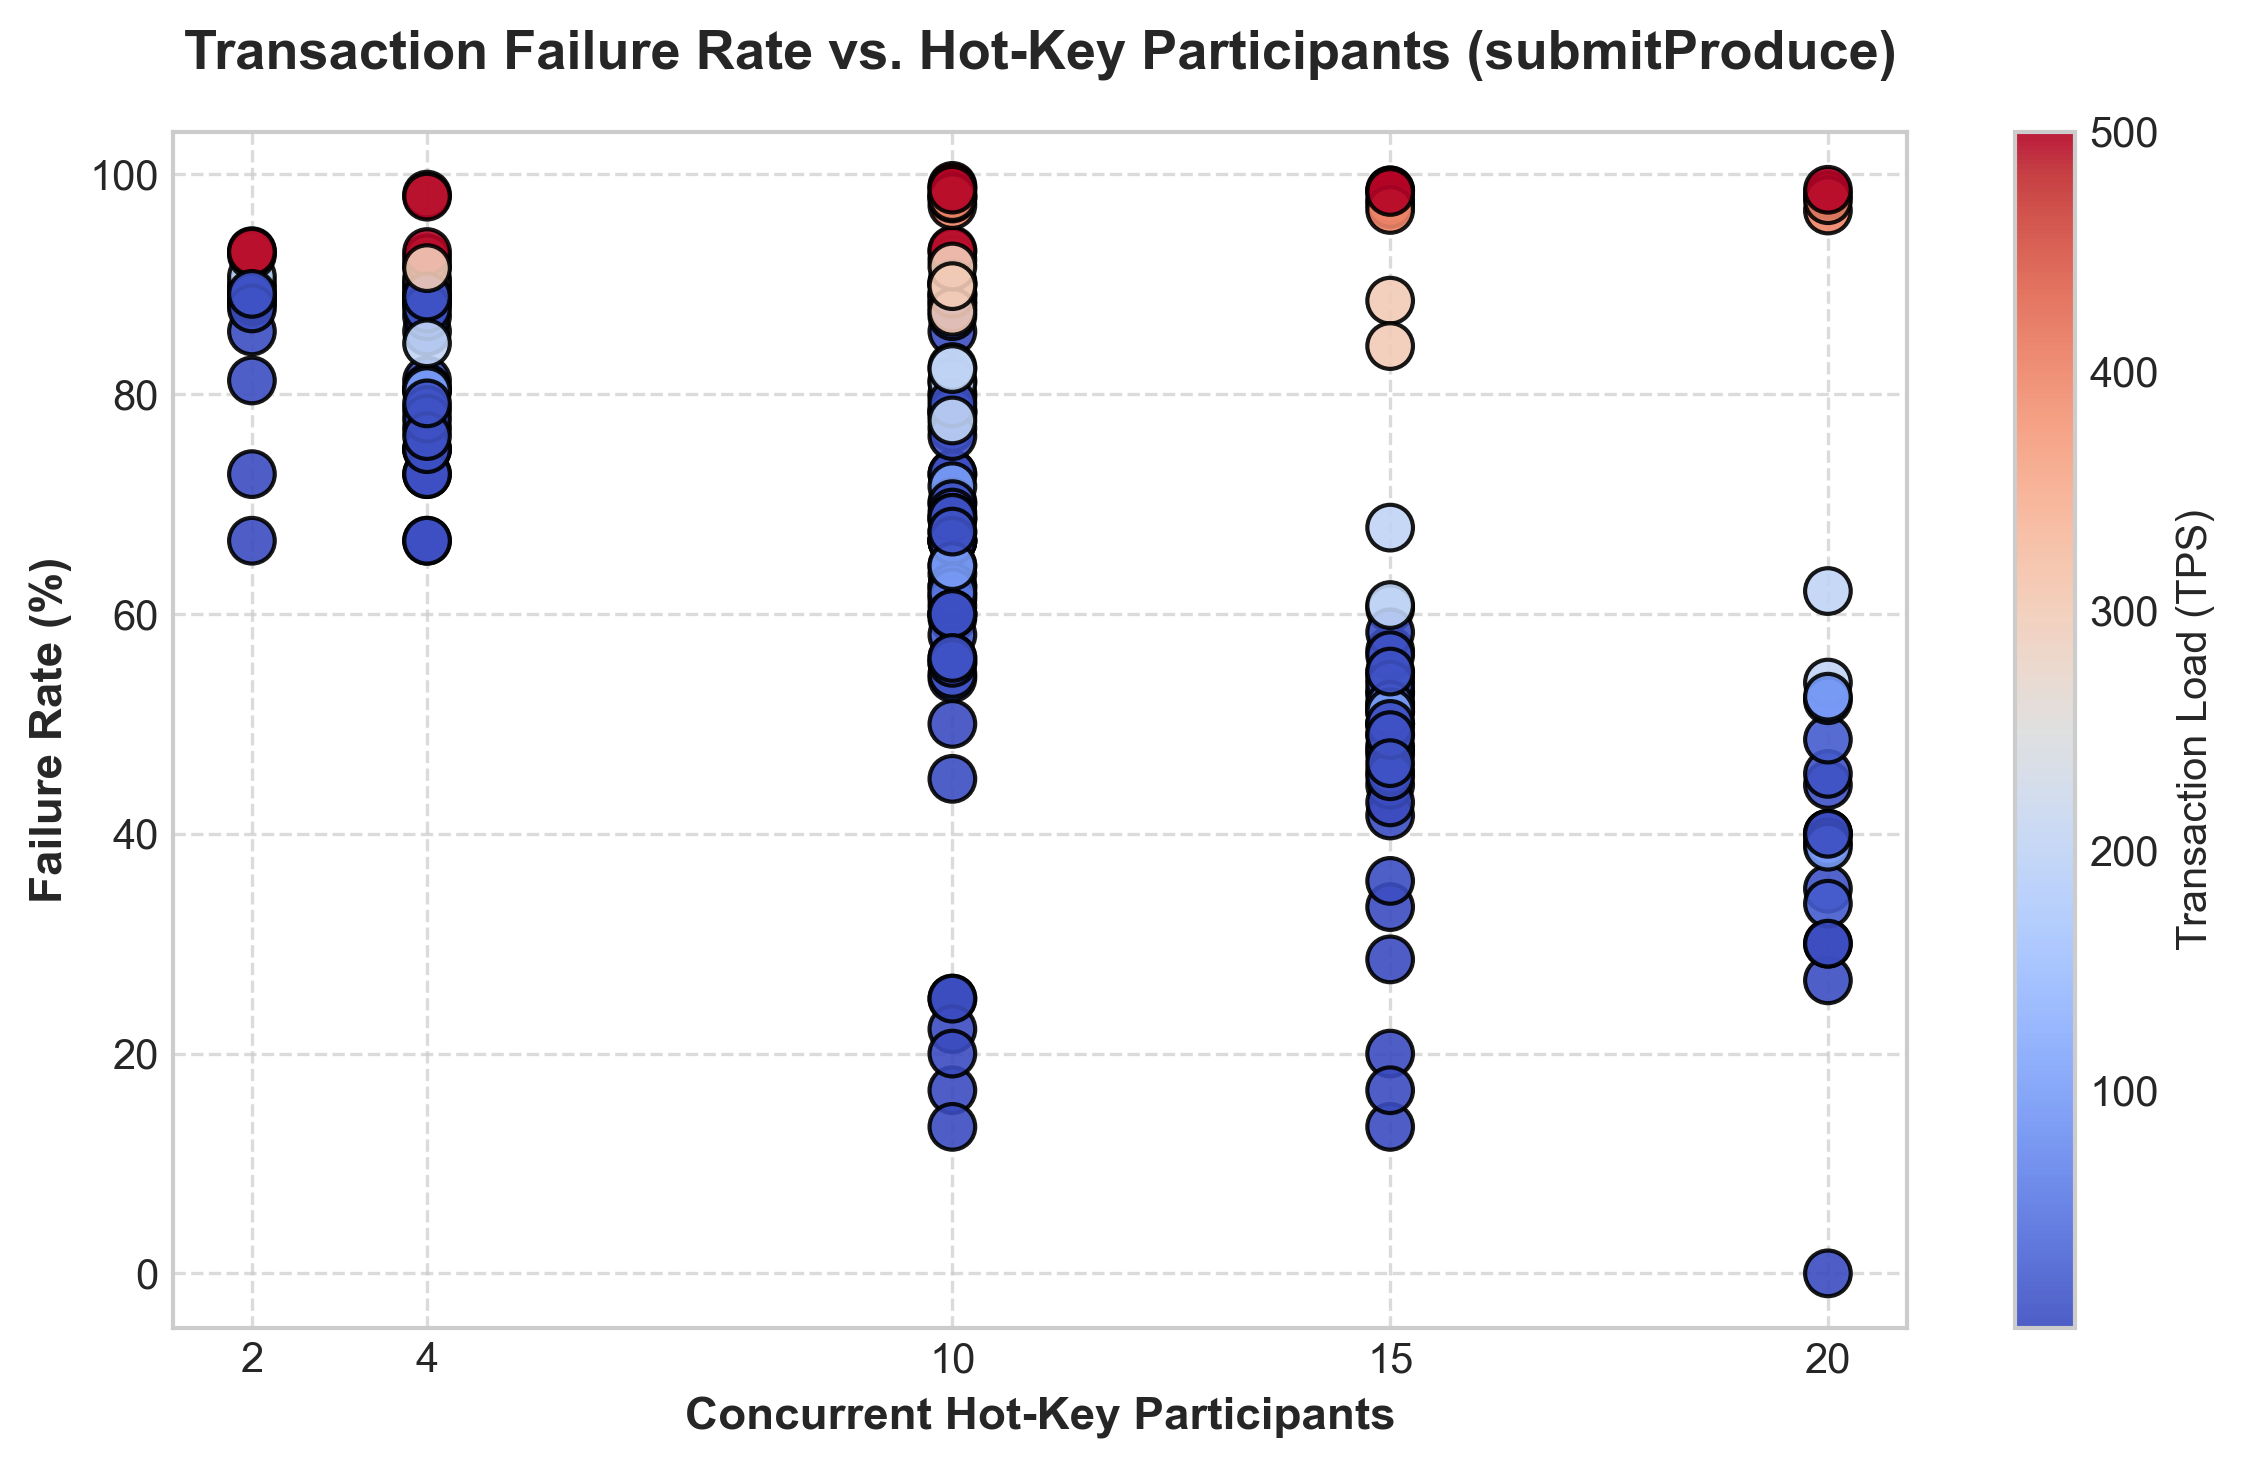
\includegraphics[width=\textwidth]{failures_vs_hotkeys_submitproduce.png}
        \caption{submitProduce}
    \end{minipage}
    
    \vspace{0.3cm}
    
    \begin{minipage}[b]{0.48\textwidth}
        \centering
        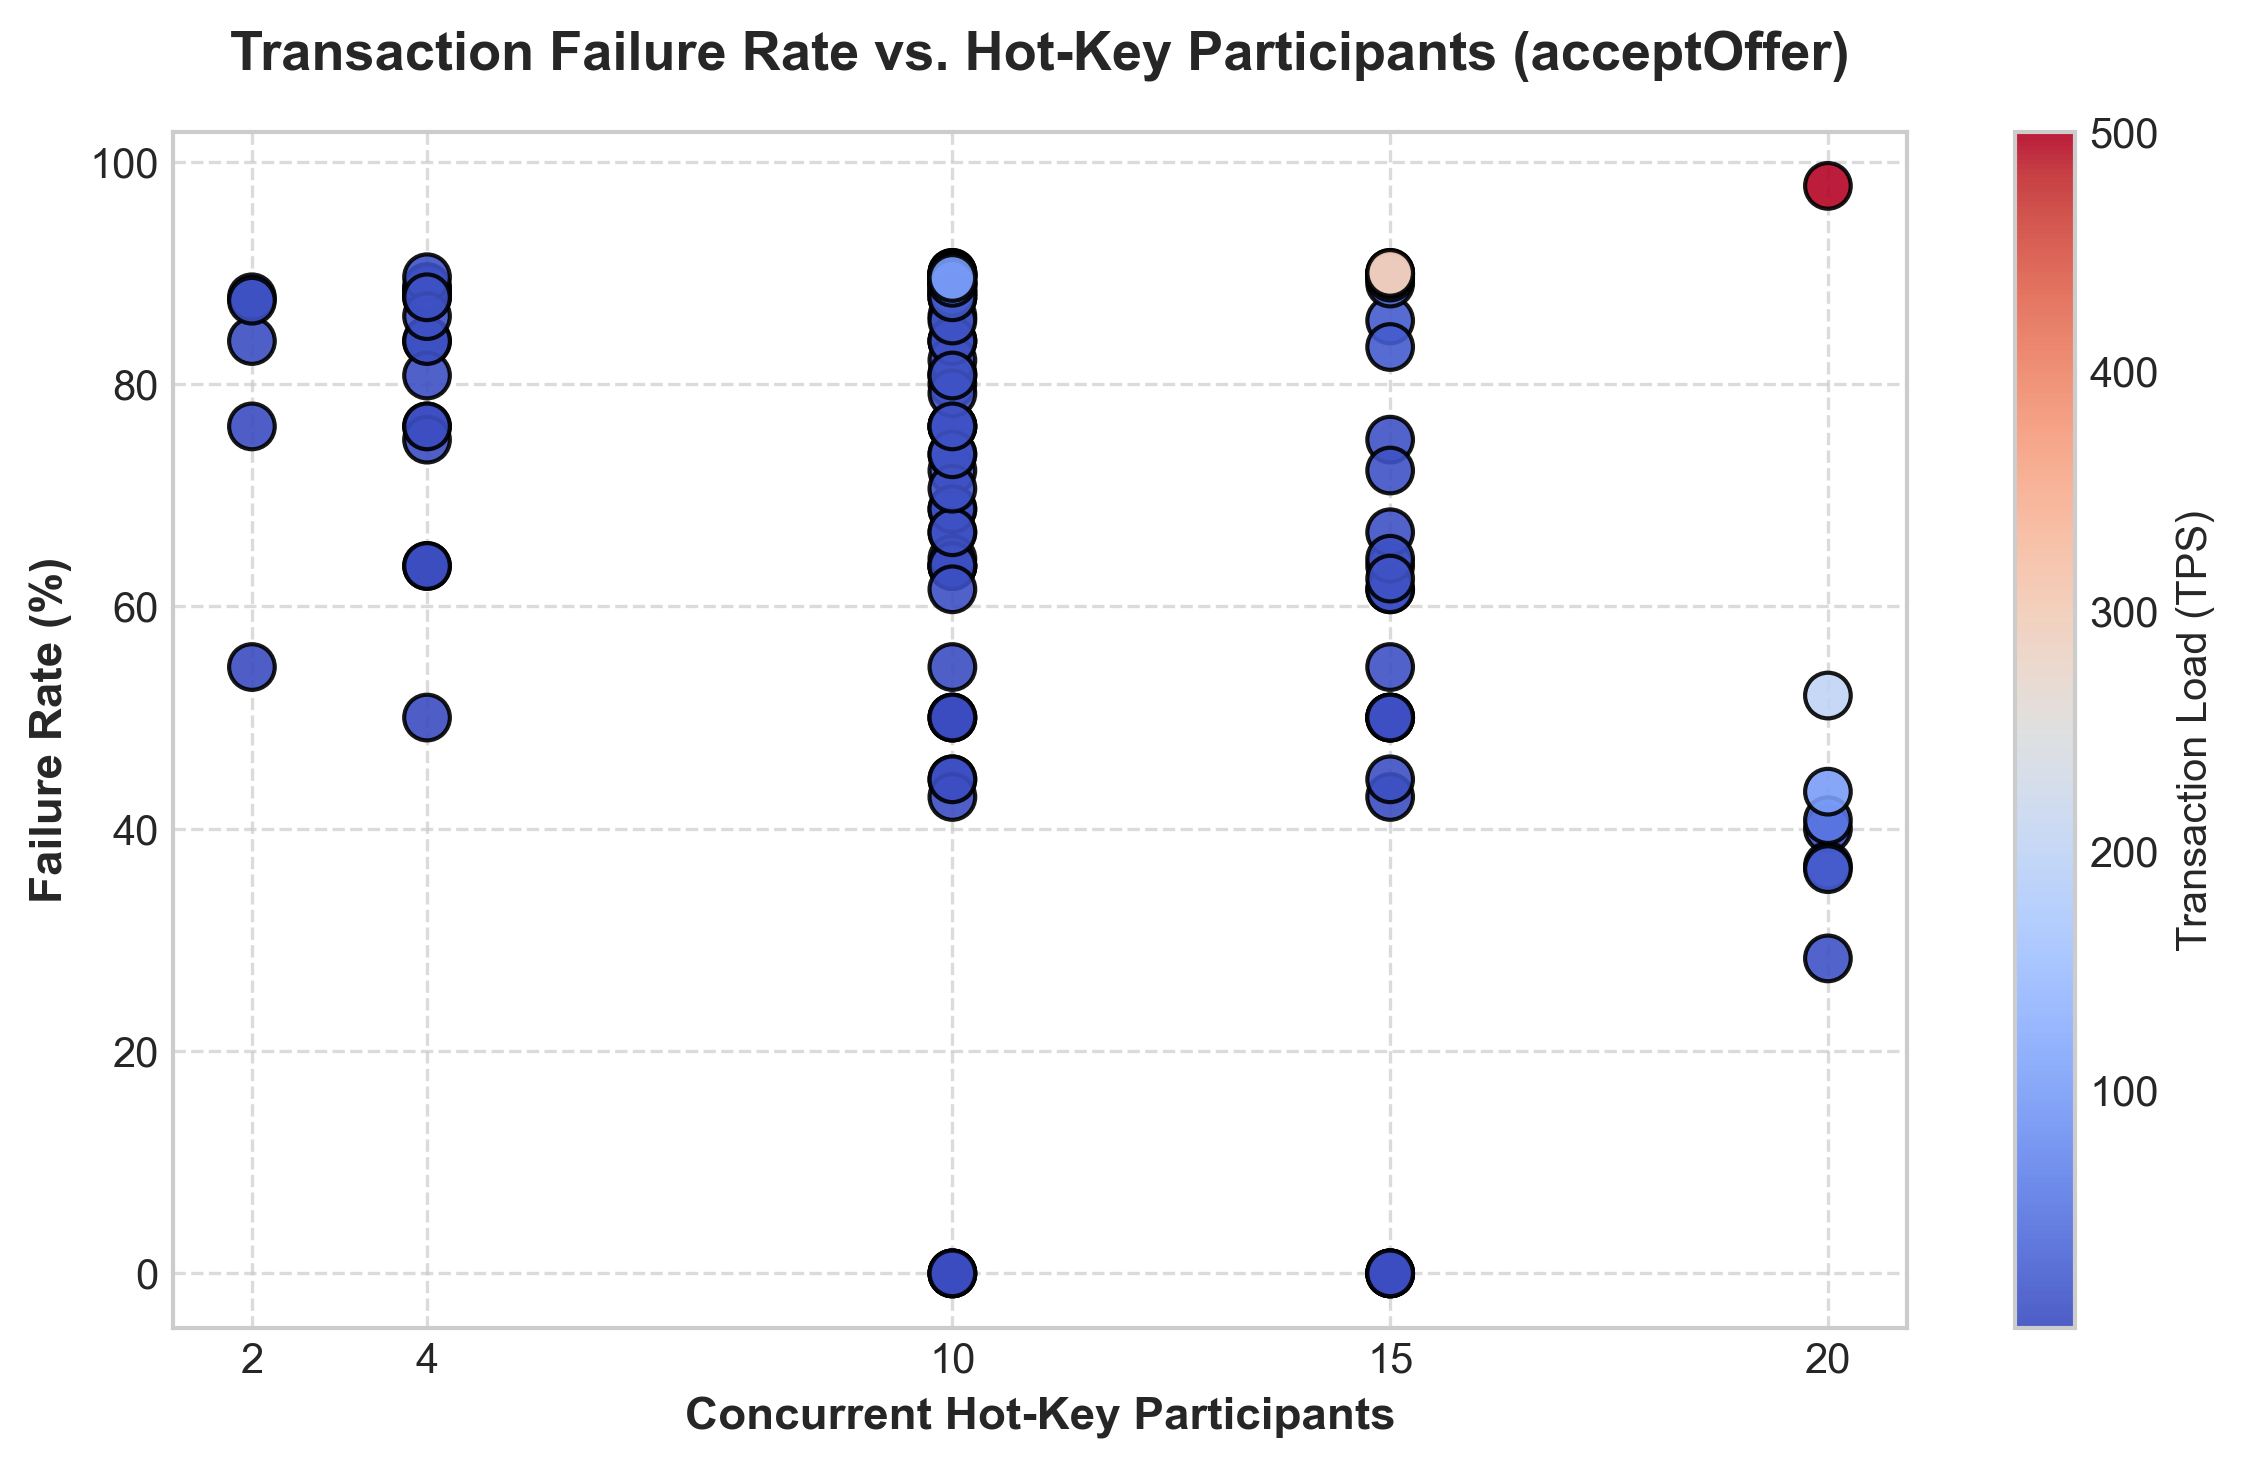
\includegraphics[width=\textwidth]{failures_vs_hotkeys_acceptoffer.png}
        \caption{acceptOffer}
    \end{minipage}
    \hfill
    \begin{minipage}[b]{0.48\textwidth}
        \centering
        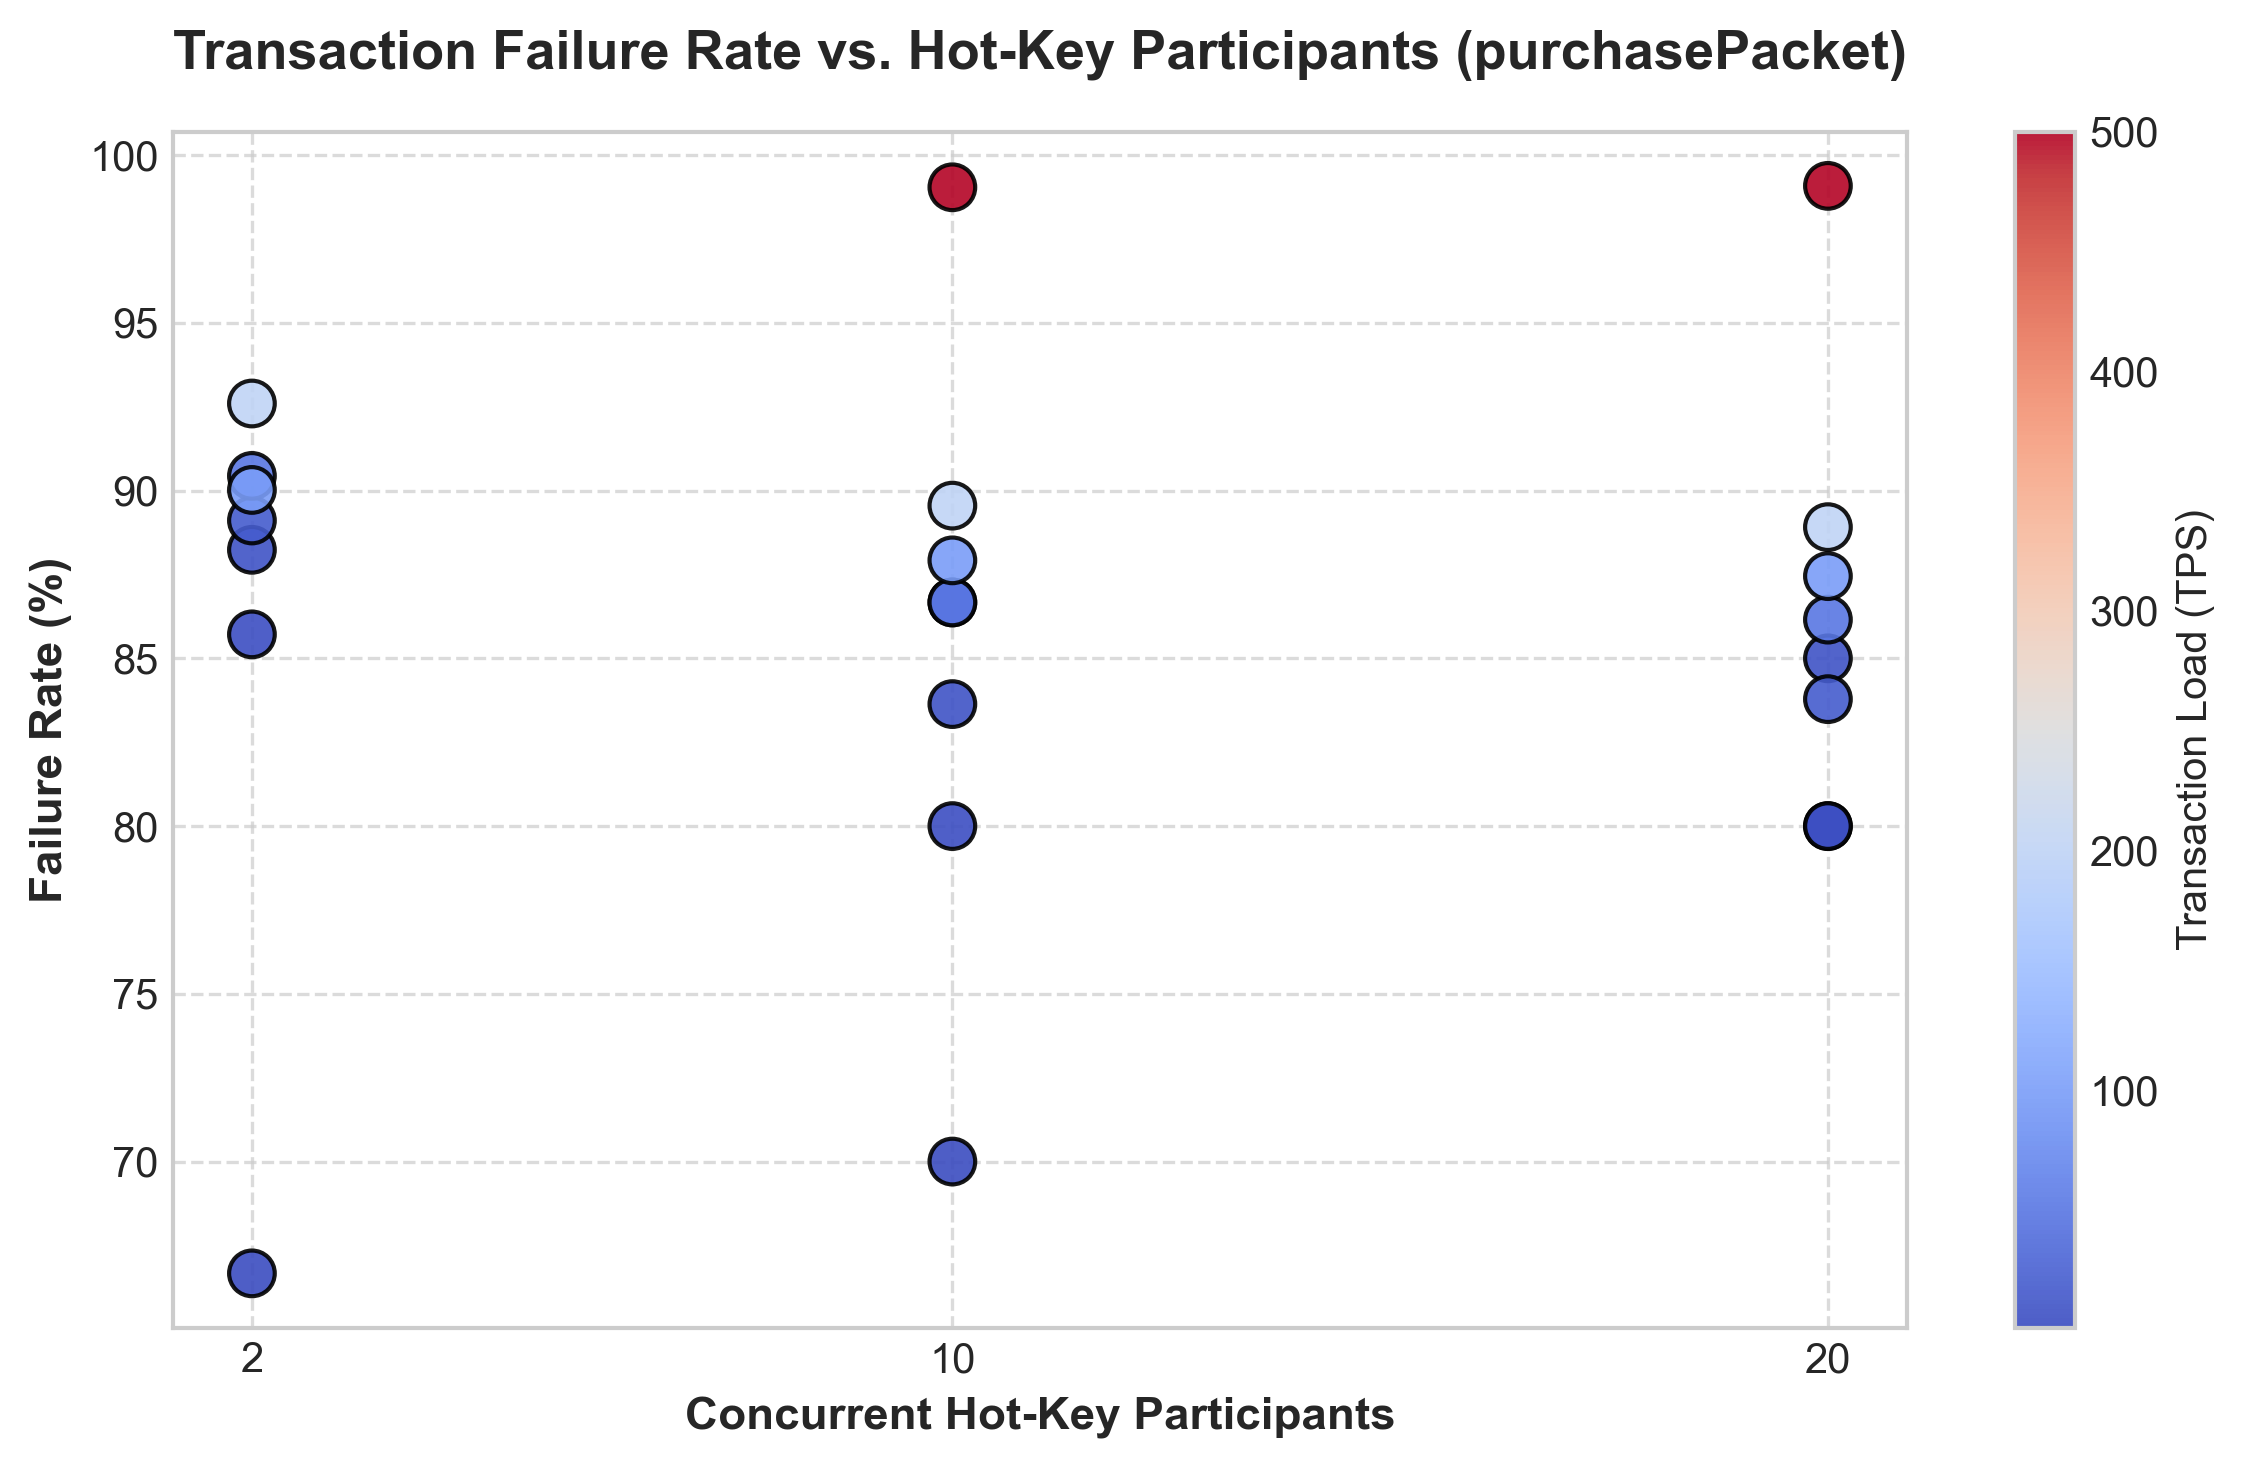
\includegraphics[width=\textwidth]{failures_vs_hotkeys_purchase.png}
        \caption{purchasePacket}
    \end{minipage}
    \caption{Empirical transaction failure rates scaling in direct proportion to the number of concurrent hot-key participants.}
    \label{fig:hotkey_failures}
\end{figure}


\subsection{Predictive Benchmarking}

While empirical benchmarking identifies the hard performance ceilings of the supply chain smart contracts, transaction failures within permissioned blockchains are driven by complex, non-linear interactions between transaction load, participant counts, ledger read/write complexities, and network conditions. To mathematically map these failure triggers, we extracted the Hyperledger Caliper transaction logs and trained predictive machine learning models. The models were trained on a strategic participant matrix (1 to 24 peers) under varying fixed-rate TPS loads (1 to 500) across all primary chaincode functions.

\subsubsection{Evaluated Predictive Architectures}
To validate the hypothesis that MVCC conflicts scale non-linearly and exhibit strict threshold "cliffs" based on structural topology, four regression architectures were evaluated: Linear Regression, Gradient Boosting, Random Forest, and a Random Forest ensemble. The empirical performance of these predictive architectures was evaluated for both successful transaction throughput and the transaction failure rate. 

As mathematically proven by the $R^2$ scores across both prediction targets, the baseline linear architecture (Linear Regression) failed to accurately model the non-linear distributions, particularly for failure rates ($\sim0.61~R^2$). This explicitly validates the hypothesis that blockchain MVCC saturation induces severe, non-linear performance cliffs rather than gradual linear degradation. Conversely, tree-based ensemble architectures (Random Forest) captured over $92\%$ of the variance for both throughput and failure rates. \textbf{Random Forest} was explicitly selected as the primary analytical framework for this study. Random Forest's independent bagging mechanism provides a more balanced and robust distribution of feature importance across highly correlated variables, avoiding the aggressive, single-feature dominance often exhibited by sequential boosting models.

\subsubsection{Throughput Prediction}
Table \ref{tab:throughput_performance} details the empirical performance of the predictive architectures when tasked with modeling the network's Transaction Throughput.

\begin{table}[ht]
\centering
\caption{Comparative Predictive Performance (Target: Transaction Throughput)}
\label{tab:throughput_performance}
\resizebox{0.8\columnwidth}{!}{%
\begin{tabular}{|l|c|c|c|}
\hline
\textbf{Machine Learning Model} & \textbf{$R^2$ Score} & \textbf{MAE} & \textbf{RMSE} \\
\hline
Linear Regression & 0.8140 & 17.497 & 30.257 \\
Gradient Boosting & 0.9142 & 8.339 & 20.541 \\
\textbf{Random Forest Regressor} & \textbf{0.9298} & \textbf{6.001} & \textbf{18.580} \\

\hline
\end{tabular}%
}
\end{table}

The trained Random Forest model demonstrated robust generalization for throughput prediction. As shown in Figure \ref{fig:throughput-feature-importance}, the model confirmed that the raw \textbf{Transaction Send Rate (Load)} is the overwhelming constraint on successful throughput, absorbing an incredible $87.8\%$ of the predictive importance. Unlike failure events, successful throughput is primarily dictated by raw network pressure rather than structural smart contract complexity.

\begin{figure}[ht]
\centering
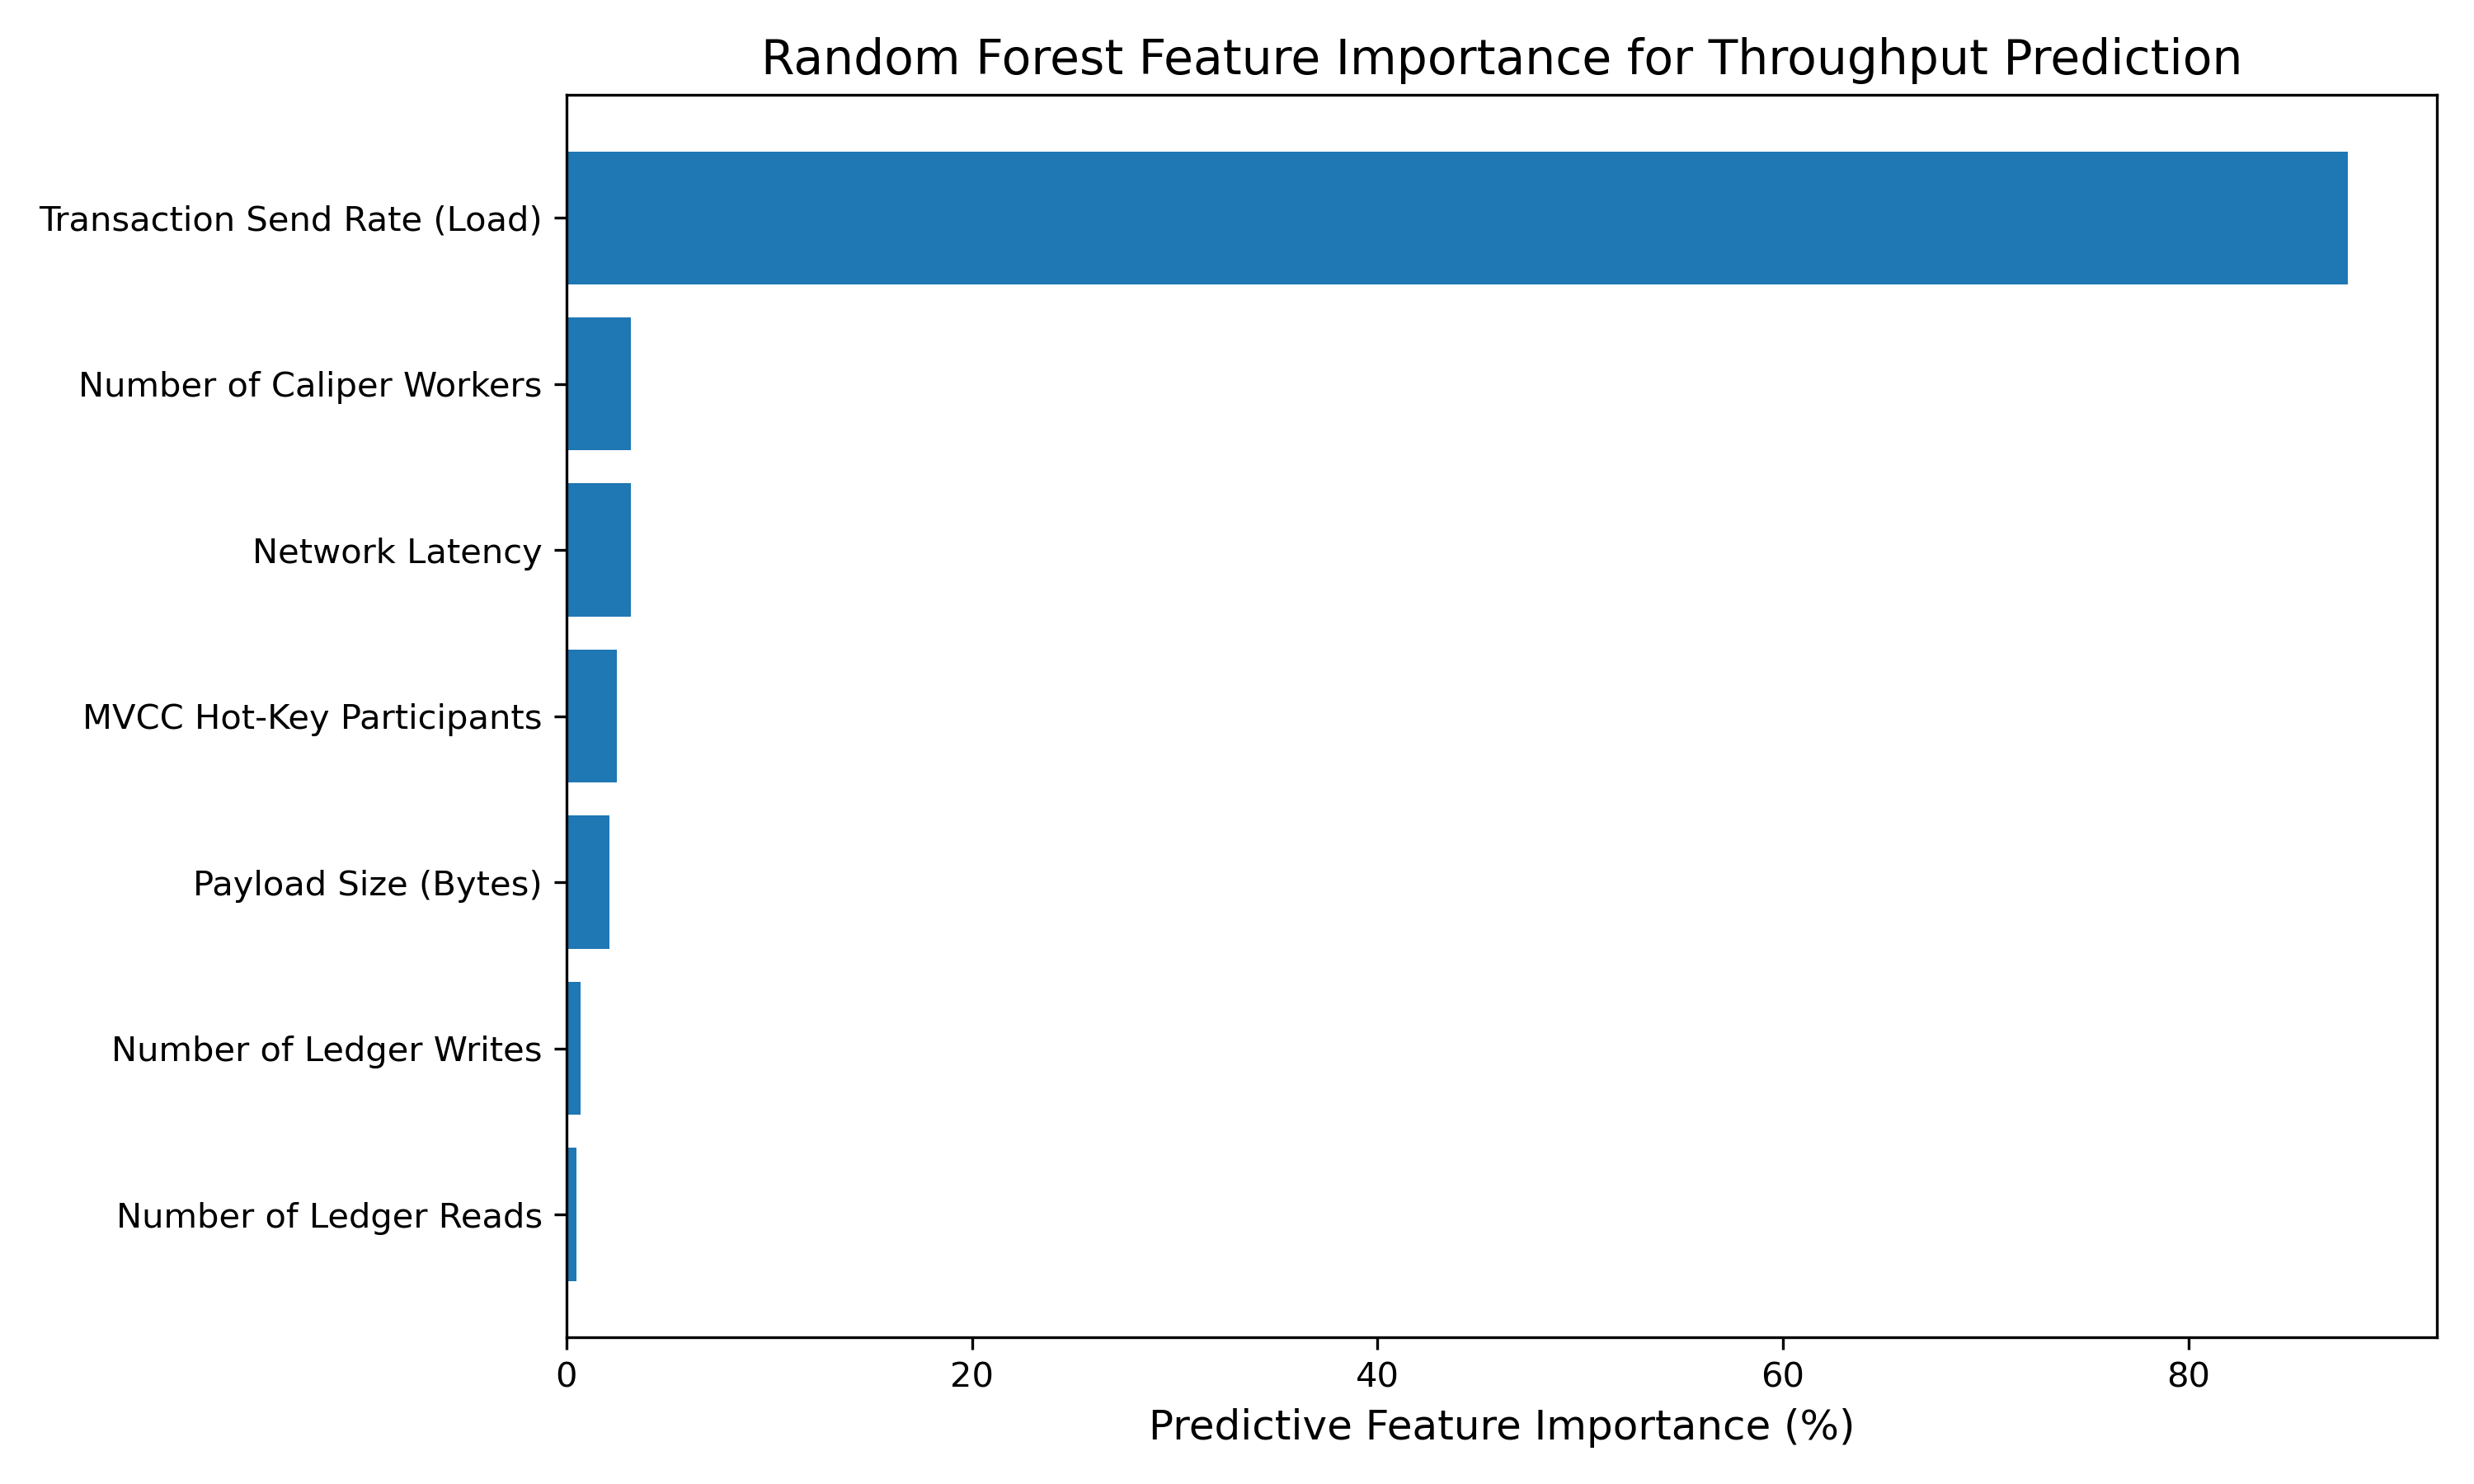
\includegraphics[width=0.8\textwidth]{throughput_feature_importance.png}
\caption{Random Forest Feature Importance ranking the dominant variables that constrain successful transaction throughput.}
\label{fig:throughput-feature-importance}
\end{figure}

\subsubsection{Failure Prediction and Feature Importance}
Table \ref{tab:failure_performance} details the empirical performance of the architectures when tasked with modeling the Transaction Failure Rate.

\begin{table}[ht]
\centering
\caption{Comparative Predictive Performance (Target: Transaction Failure Rate)}
\label{tab:failure_performance}
\resizebox{0.8\columnwidth}{!}{%
\begin{tabular}{|l|c|c|c|}
\hline
\textbf{Machine Learning Model} & \textbf{$R^2$ Score} & \textbf{MAE} & \textbf{RMSE} \\
\hline
Linear Regression & 0.6180 & 0.158 & 0.216 \\
Gradient Boosting & 0.9094 & 0.070 & 0.105 \\
\textbf{Random Forest Regressor} & \textbf{0.9602} & \textbf{0.032} & \textbf{0.069} \\

\hline
\end{tabular}%
}
\end{table}

The trained Random Forest model successfully mapped the complex, multi-factorial catalysts responsible for transaction timeouts and Multi-Version Concurrency Control (MVCC) \texttt{READ\_CONFLICT} errors. As shown in Figure \ref{fig:feature-importance}, transaction failures are driven by a distributed combination of state-contention and network stress. \textbf{MVCC Hot-Key Participants} ($23.1\%$), raw \textbf{Transaction Load} ($20.7\%$), \textbf{Number of Ledger Reads} ($18.8\%$), and \textbf{Payload Size} ($17.1\%$) collectively dictate the failure rate. This balanced feature distribution mathematically proves that MVCC failures cannot be attributed to a single bottleneck; rather, they occur when dense participant state-traversals collide simultaneously with high network data volumes.

\begin{figure}[ht]
\centering
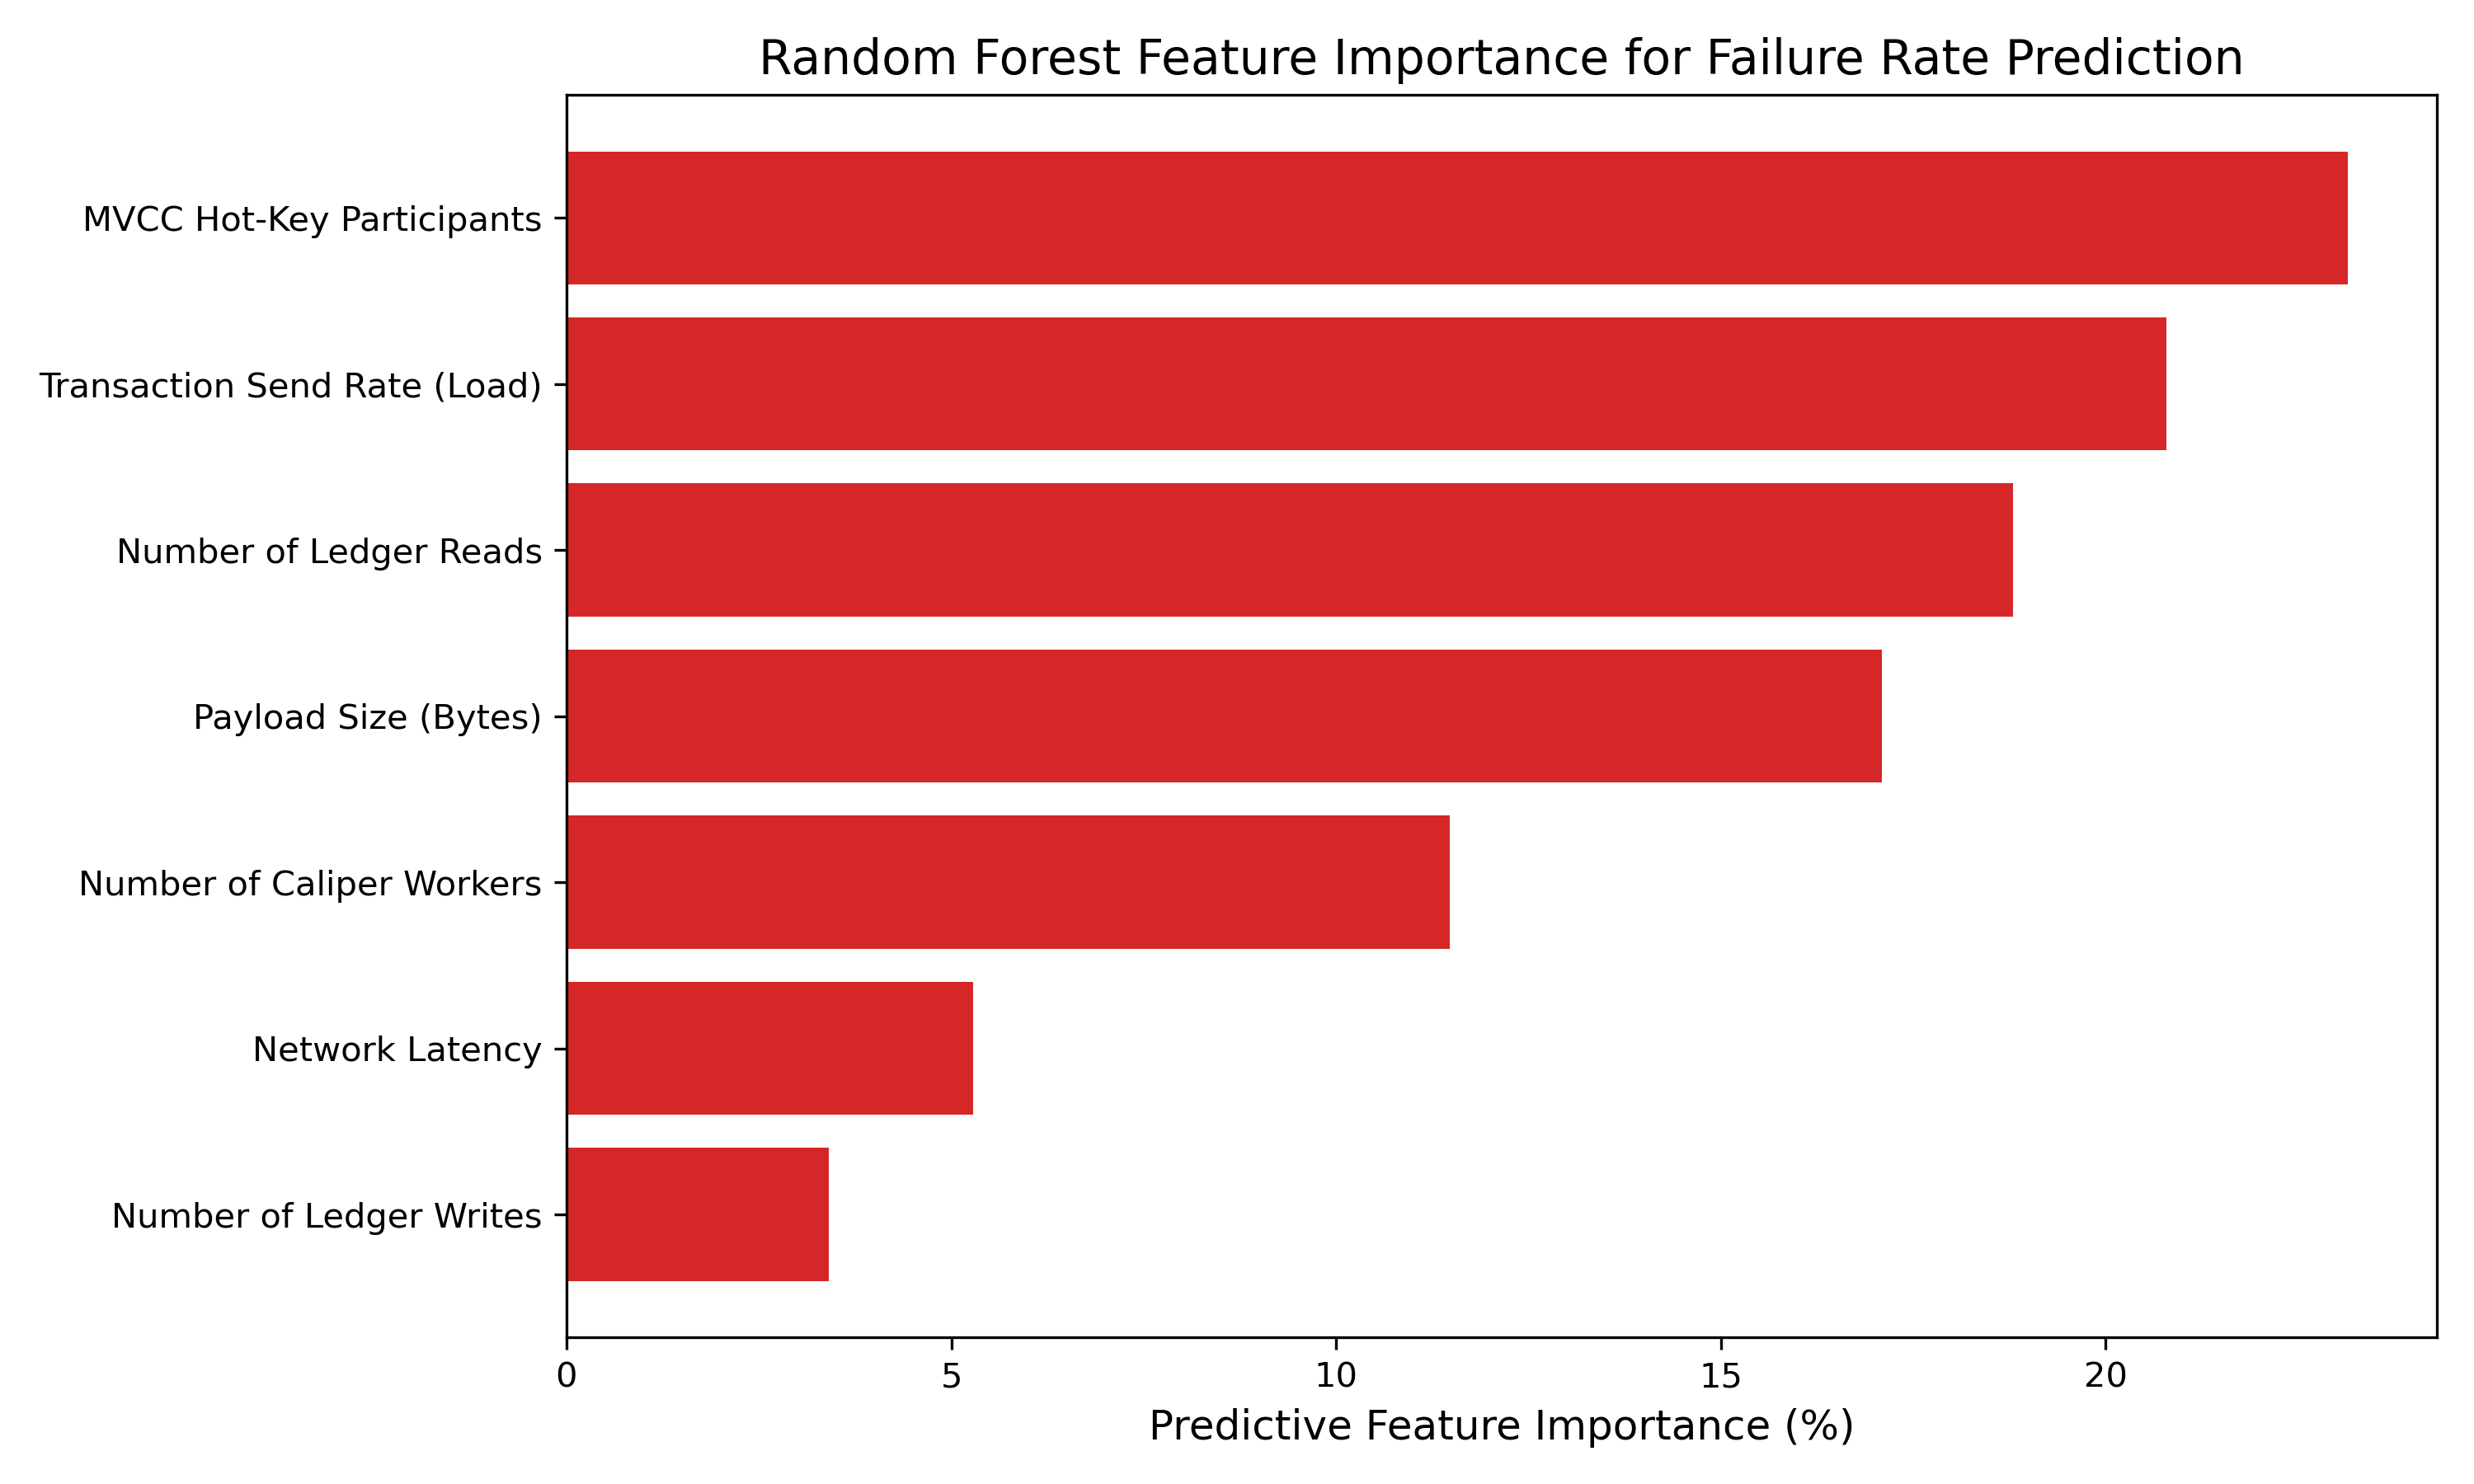
\includegraphics[width=0.8\textwidth]{chart_feature_importance.png}
\caption{Random Forest Feature Importance ranking the distributed variables that trigger transaction failures.}
\label{fig:feature-importance}
\end{figure}

To understand \textit{how} these variables push the Hyperledger orderer and endorser nodes toward failure, we computed SHapley Additive exPlanations (SHAP) values. Figure \ref{fig:shap-summary} presents the SHAP summary plot, which explicitly proves the directional relationship: high transaction loads (red dots) heavily push the model toward predicting a higher failure rate (positive SHAP value), whereas lightweight transactions with low participant counts push the model toward a 100\% success rate (negative SHAP value).

\begin{figure}[ht]
	\centering
	\begin{minipage}[b]{0.48\textwidth}
		\centering
		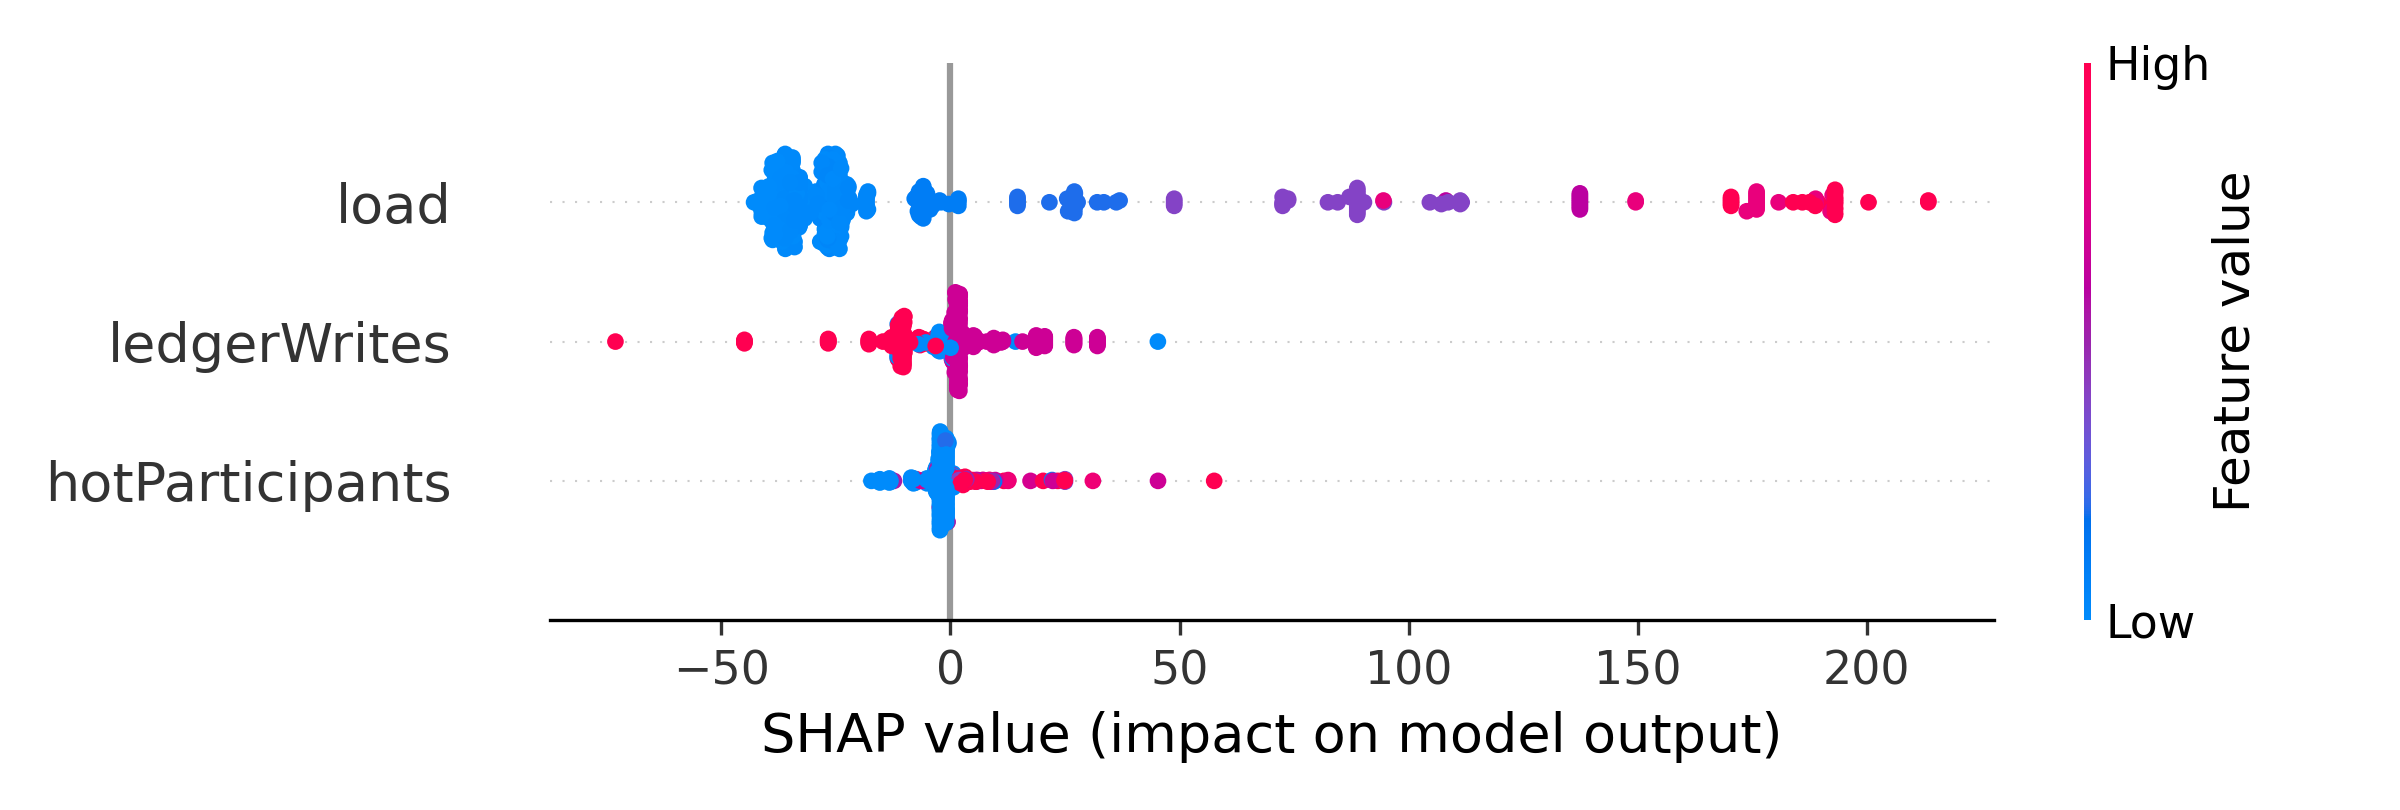
\includegraphics[width=\textwidth]{chart_shap_summary.png}
		\caption{SHAP Summary Plot demonstrating the directional impact of concurrent load and function complexity on transaction failures.}
		\label{fig:shap-summary}
	\end{minipage}
	\hfill
	\begin{minipage}[b]{0.48\textwidth}
		\centering
		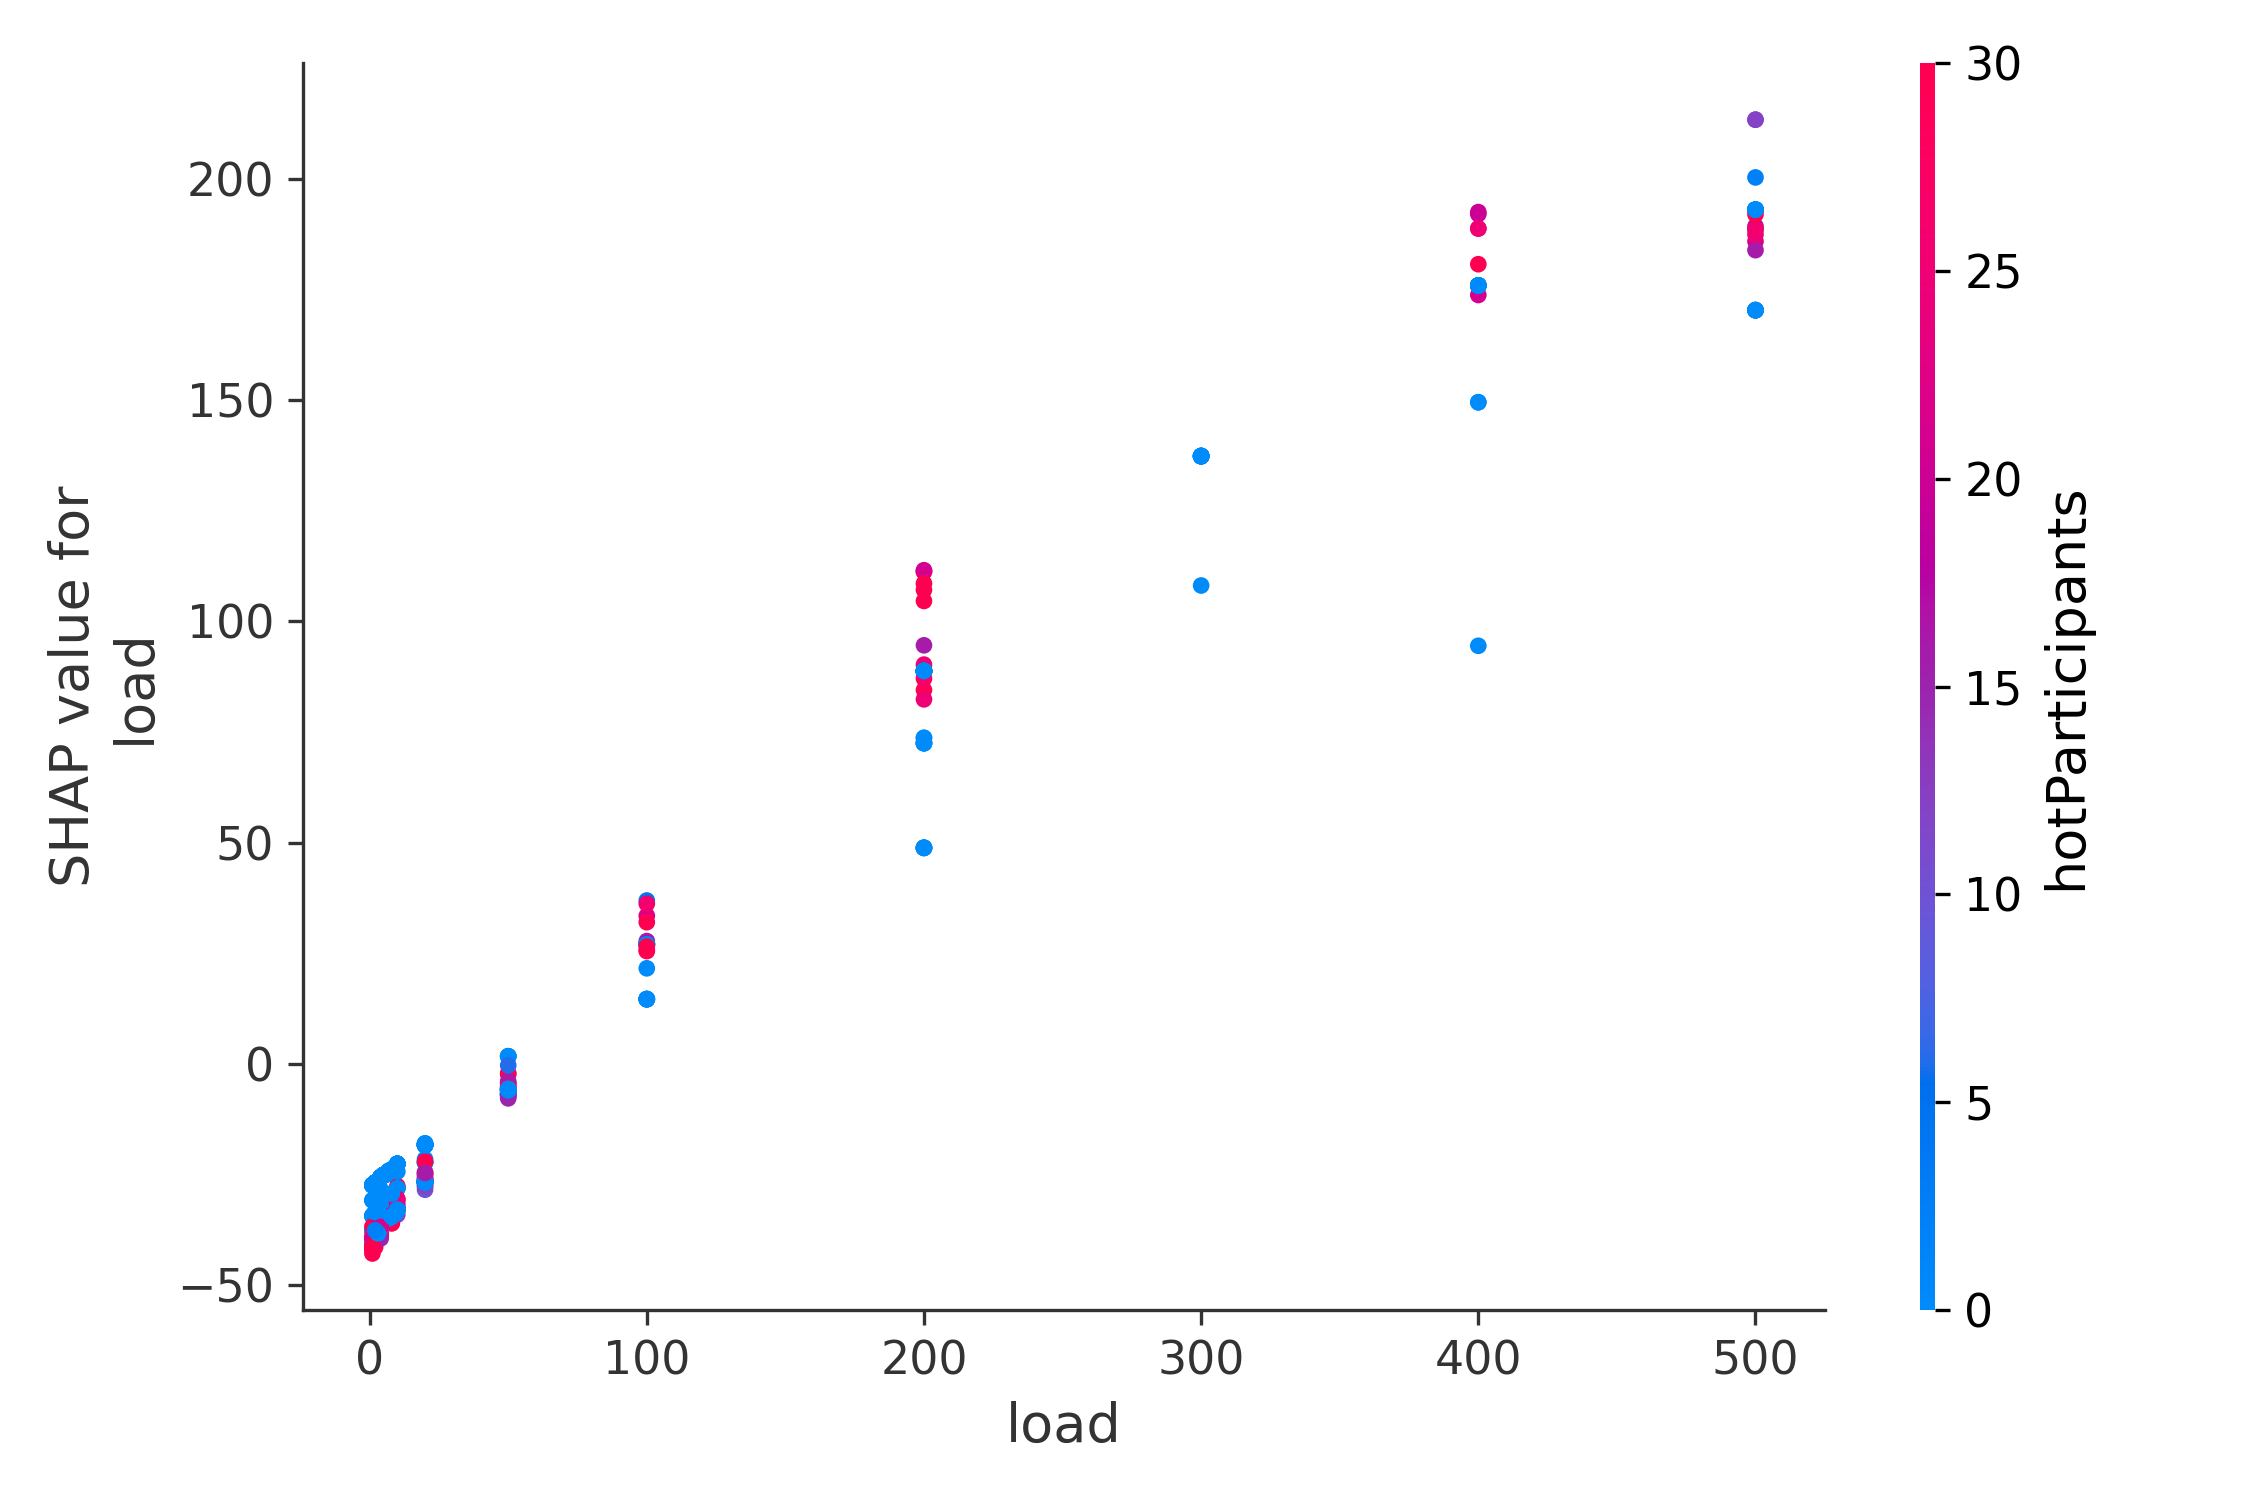
\includegraphics[width=\textwidth]{chart_shap_dependence.png}
		\caption{SHAP Dependence Plot highlighting the non-linear interaction between load and participant counts.}
		\label{fig:shap-dependence}
	\end{minipage}
\end{figure}

The SHAP Dependence plot (Figure \ref{fig:shap-dependence}) further highlights the severe non-linear bottlenecks present in the unoptimized smart contract architecture. As concurrent TPS increases, the likelihood of a transaction encountering a stale read or timeout increases exponentially. This predictive modeling validates the necessity for architectural refactoring---such as implementing append-only partial composite keys---to decouple state writes and mitigate concurrent hot-key collisions.


\section{Conclusion}
	
	This study set out to address a fundamental challenge in the practical deployment of permissioned blockchain systems: the difficulty of predicting and diagnosing non-linear Multi-Version Concurrency Control (MVCC) failures before they cause catastrophic throughput degradation in production environments. Using a Hyperledger Fabric-based agricultural supply chain system as a real-world empirical testbed, we developed and validated a machine learning framework---based on a Random Forest ensemble---that accurately forecasts both MVCC failure rates and transaction throughput from interpretable structural and operational features.

The performance analysis, conducted via Hyperledger Caliper across 11 send-rate levels and a comprehensive participant matrix, revealed severe MVCC-induced throughput degradation in functions with shared wallet keys (	extit{submitProduce}, 	extit{acceptOffer}, 	extit{purchasePacket}) and shared lot state (	extit{makeOffer}). Critically, the Random Forest predictive model demonstrated that failures are a distributed phenomenon driven by a combination of 	extbf{MVCC Hot-Key Participants} ($23.1\%$), 	extbf{Transaction Load} ($20.7\%$), and 	extbf{Number of Ledger Reads} ($18.8\%$). Conversely, for throughput prediction, the 	extbf{Transaction Send Rate (Load)} was the overwhelming constraint, absorbing an incredible $87.8\%$ of the predictive importance. These findings mathematically prove that while throughput is dictated by raw network pressure, MVCC failures occur when dense participant state-traversals collide simultaneously with high network data volumes.

The results confirm that append-only, composite-key-based chaincode designs substantially reduce MVCC conflicts, and that the Random Forest model provides an accurate, interpretable diagnostic tool for identifying which chaincode functions and participant configurations are at highest risk. Looking ahead, future work will extend this predictive framework to distributed multi-host deployments with wide-area network conditions, explore dynamic chaincode optimization strategies guided by model predictions, and integrate real-time IoT sensor data streams for objective quality grading. The supply chain finance layer can be extended with weather-indexed smart contract insurance and credit access mechanisms leveraging verified on-chain transaction histories, further strengthening the financial resilience and scalability of agri-food blockchain deployments.
	
		
	\section*{Declaration of generative AI and AI-assisted technologies in the writing process}
	During the preparation of this work the author(s) used \textbf{DeepL} and \textbf{ChatGPT} in order to improve language and readability. 
	After using these tools, the author(s) reviewed and edited the content as needed and take full responsibility for the content of the publication.
	
	\section*{CRediT authorship contribution statement}
	% Replace with your actual author names and roles
	Dhanish Jose: Writing – original draft, Writing – review \& editing, Validation, Methodology, Conceptualization.\\
	Pradeepmon T G: Writing – review \& editing, Validation, Resources, Supervision.
	
	
	\section*{Declaration of competing interest}
	The authors declare that they have no known competing financial interests or personal relationships 
	that could have appeared to influence the work reported in this paper.
	
	\section*{Data availability}
	Data will be made available on request.
	
	\section*{Acknowledgements}
	This work was supported by \textbf{National Institute of Technology Calicut (NIT Calicut)}.
	
	
	\appendix
	

	
	
	\bibliography{references}
	% <-- REQUIRED line
	
\end{document}
